% Relatório do artefato computacional. Proposta.tex permanece como histórico.
\documentclass[alpha-refs,english,brazilian]{CC-EC_TF-TC}
\usepackage{tikz}
\usetikzlibrary{arrows.meta,positioning,fit,shapes.geometric}

\AtBeginDocument{\renewcommand{\harvardand}{e}}
% Inclui apenas capturas reais existentes. IDs/contextos ficam no inventário.
\newcommand{\capturatcc}[4]{%
  \IfFileExists{fig/capturas/#1.png}{%
    \begin{figure*}[htbp]
      \centering
      \includegraphics[width=0.94\textwidth,height=0.40\textheight,keepaspectratio]{fig/capturas/#1.png}
      \caption{#3. Fonte: execução local e arquivos gerados.}
      \label{fig:#1}
    \end{figure*}%
  }{}%
}

\hypersetup{pdftitle={Sistema de Monitoramento Agrícola por Imagens de Satélite},pdfauthor={Eduardo Steffens Hoppen},pdfsubject={Trabalho de Conclusão de Curso - Ciência da Computação - UPF}}

\title{Sistema de Monitoramento Agrícola por Imagens de Satélite}
\titleother{Agricultural Monitoring System Using Satellite Imagery}
\author[1]{Eduardo Steffens Hoppen}
\affil[1]{Universidade de Passo Fundo, Instituto de Tecnologia, Curso de Ciência da Computação\\Orientador: Prof. Carlos Amaral Holbig}
\runningauthor{Hoppen}
\titulores{Monitoramento agrícola por imagens de satélite}
\papercat{Trabalho de Conclusão de Curso}
% PENDENTE: confirmar mês e ano da defesa.
\jyear{2026}
\jmonth{} % Pendente administrativo: mês da defesa, confirmar antes da entrega.
\jcourse{Ciência da Computação}
\setcounter{page}{1}
\firstpage{1}

\begin{document}
\begin{frontmatter}
\maketitle
\thispagestyle{empty}
\begin{Abstract}
\selectlanguage{english}
Integrating satellite imagery into agricultural software requires consistency across geometries, dates, units and outputs. This study developed and technically assessed a modular web platform using Python, Streamlit, Google Earth Engine, Sentinel-2 and NASA POWER. Development followed a specification-driven workflow. The platform computes the Normalized Difference Vegetation Index (NDVI) and near-infrared--shortwave-infrared variants labelled Normalized Difference Water Index (NDWI) and Normalized Difference Moisture Index (NDMI). It integrates maps, time series, weather data, browser-side grid queries and exports. The documented assessment recorded 710 passing Python tests, 100\% line and branch coverage in the measured modules, three JavaScript checks and a demonstration with real services. A completed exploratory questionnaire with \UsuariosN{} responses yielded a mean rating of \UsuariosMediaEN{}/10, a median of \UsuariosMediana{} and barriers involving area selection and alert interpretation. The contribution lies in data integration, state consistency and traceable outputs. The evidence supports the demonstrated computational workflow; the questionnaire describes self-reported use, without population-level generalization. Agronomic field validation and calibration of the temporal heuristics remain future work.
\end{Abstract}
\begin{keywords}
software engineering; agricultural monitoring; remote sensing; geospatial processing; data visualization.
\end{keywords}
\selectlanguage{brazilian}

\begin{resumo}
Integrar imagens de satélite a um software agrícola exige consistência entre geometrias, datas, unidades e saídas. Este estudo desenvolveu e avaliou tecnicamente uma plataforma web modular com Python, Streamlit, Google Earth Engine, Sentinel-2 e NASA POWER. O desenvolvimento seguiu um fluxo orientado a especificações. A plataforma calcula o índice de vegetação por diferença normalizada (NDVI) e variantes infravermelho próximo--infravermelho de ondas curtas denominadas índice de água por diferença normalizada (NDWI) e índice de umidade por diferença normalizada (NDMI). Integra mapas, séries temporais, dados meteorológicos, consulta a grades no navegador e exportações. A avaliação documentada registrou 710 testes Python aprovados, com 100\% de cobertura de linhas e ramificações nos módulos medidos, três verificações JavaScript e demonstração com serviços reais. O questionário exploratório concluído, com \UsuariosN{} respostas, apresentou nota média de \UsuariosMedia{}/10, mediana \UsuariosMediana{} e barreiras de demarcação e interpretação de alertas. A contribuição está na integração de dados, na coerência do estado e na rastreabilidade das saídas. As evidências sustentam o fluxo computacional demonstrado; o questionário descreve o uso autodeclarado, sem generalização populacional. Validação agronômica em campo e calibração das heurísticas temporais permanecem como trabalhos futuros.
\end{resumo}
\begin{palavras_chave}
engenharia de software; monitoramento agrícola; sensoriamento remoto; processamento geoespacial; visualização de dados.
\end{palavras_chave}

\end{frontmatter}
\clearpage

\section{Introdução}\label{chap:introducao-final}

Para acompanhar uma área agrícola, é importante observar tanto as diferenças entre suas partes quanto as mudanças que ocorrem ao longo do tempo. Imagens multiespectrais de satélites registram a superfície em diferentes faixas do espectro, permitindo calcular indicadores associados à vegetação e à umidade. A literatura descreve aplicações agrícolas com diferentes sensores, escalas e métodos de interpretação \citep{WEISS2020}. Porém, ter acesso às imagens não basta para utilizá-las em uma aplicação. Ainda é necessário delimitar a área, consultar as imagens do período, selecionar as bandas, tratar observações inválidas e organizar os resultados.

Para explorar esses dados em uma aplicação, não basta calcular um índice. O mapa, o gráfico e os arquivos exportados precisam corresponder à área e ao período escolhidos pelo usuário. Essa integração exige cuidado porque as imagens de satélite podem estar disponíveis em datas irregulares, enquanto as informações meteorológicas são organizadas por dia. É necessário, portanto, definir como cada parte do sistema trata a área selecionada, as datas, as unidades de medida e os dados ausentes. Essas regras de troca e interpretação das informações, chamadas aqui de contratos de dados, também fazem parte do problema de Engenharia de Software.

O problema de pesquisa foi delimitado pela seguinte questão: como construir e verificar tecnicamente uma plataforma computacional que integre gerenciamento de áreas geográficas, índices espectrais, exploração espacial e temporal, contexto meteorológico e exportação de resultados para apoio ao monitoramento agrícola?

\subsection{Motivação, justificativa e contribuição}

O Google Earth Engine permite consultar catálogos e processar imagens em sua infraestrutura remota. Já o projeto Prediction Of Worldwide Energy Resources (POWER), da NASA, disponibiliza informações meteorológicas e de radiação que podem ser consultadas pelo software \citep{GORELICK2017,NASA_POWER_DAILY}. Com esses serviços, a aplicação não precisa manter uma infraestrutura própria de distribuição de imagens. Ainda assim, precisa organizar as consultas, tratar a indisponibilidade dos serviços e apresentar cada resultado junto da área, do período e dos parâmetros usados para produzi-lo.

A contribuição deste trabalho consiste em reunir técnicas já conhecidas em uma plataforma e documentar como elas são integradas. O usuário delimita uma área no mapa por meio de um polígono, escolhe o período e consulta os índices. A partir desses resultados, pode observar diferenças dentro da área, acompanhar sua evolução nos gráficos, examinar quedas sinalizadas na série e consultar informações meteorológicas. Também pode exportar os resultados e salvar a área para utilizá-la novamente. A contribuição em Ciência da Computação está na organização dessas etapas e na integração entre componentes, serviços e formatos de arquivo, com métodos e limites de processamento explícitos.

Não se propõem novos índices espectrais, uma nova metodologia de diagnóstico agronômico ou a revalidação dos sensores orbitais e produtos meteorológicos. A disponibilidade pública dos dados e o uso de bibliotecas abertas também não demonstram, isoladamente, menor custo total, acessibilidade universal, facilidade de uso ou superioridade frente a sistemas comerciais. Essas afirmações exigiriam avaliações específicas.

\subsection{Objetivo geral e objetivos específicos}

O objetivo geral foi desenvolver e verificar tecnicamente uma plataforma computacional integrada de apoio ao monitoramento agrícola por imagens de satélite, disponibilizando processamento geoespacial, análise espacial e temporal, contexto meteorológico e exportação de informações.

Os objetivos específicos permitem relacionar o que foi desenvolvido às verificações apresentadas no trabalho:
\begin{enumerate}[leftmargin=3em]
    \item[\textbf{OE1}] fundamentar os métodos espectrais e definir uma organização modular para integrar interface, processamento e fontes externas;
    \item[\textbf{OE2}] disponibilizar busca geográfica, demarcação, armazenamento e recuperação de polígonos, distinguindo persistência local e armazenamento por sessão;
    \item[\textbf{OE3}] integrar imagens Sentinel-2 e implementar as formulações espectrais e os filtros espaciais, temporais e de nuvens presentes na aplicação;
    \item[\textbf{OE4}] produzir composições temporais, estatísticas espaciais e mapas temáticos com exploração interativa dos valores da grade;
    \item[\textbf{OE5}] organizar séries temporais e aplicar procedimentos explícitos de classificação de tendência e sinalização de desvios negativos;
    \item[\textbf{OE6}] integrar informações meteorológicas e explicitar suas agregações, unidades e limites de interpretação;
    \item[\textbf{OE7}] gerar relatórios PDF e dados estruturados em XLSX e CSV ZIP, além de transferir localizações em GeoJSON;
    \item[\textbf{OE8}] verificar o artefato por inspeção, testes existentes e rastreabilidade, documentando evidências, inconsistências e limitações da viabilidade técnica.
\end{enumerate}

Essa organização mantém a intenção de construir o sistema e reconhece funcionalidades incorporadas durante o desenvolvimento, sem substituir os objetivos experimentais não realizados. A avaliação reúne testes computacionais, demonstração funcional e análise descritiva das respostas de usuários, distinguindo a versão pública avaliada da versão corrigida em desenvolvimento. A diferença entre o escopo executado e os estudos por cultura previstos é discutida na \cref{chap:discussao-final}.

\subsection{Delimitação e organização do texto}

A avaliação concentra-se no funcionamento do software, na troca de dados entre suas partes e nos resultados que ele apresenta e exporta. Os índices são indicadores indiretos: uma alteração em seus valores não identifica, por si só, pragas, doenças, deficiência nutricional ou estresse hídrico. Por isso, as áreas usadas nas demonstrações servem para mostrar o funcionamento da plataforma, não para caracterizar experimentos agronômicos.

A \cref{chap:fundamentacao-final} apresenta os conceitos necessários, e a \cref{chap:metodos-final} descreve os procedimentos de desenvolvimento, processamento e avaliação. A \cref{chap:implementacao-final} explica a construção da solução, enquanto a \cref{chap:plataforma-final} relaciona seus recursos às capturas disponíveis. As \cref{chap:resultados-final,chap:discussao-final} apresentam as evidências de funcionamento, o atendimento aos objetivos e seus limites. Por fim, a \cref{chap:conclusao-final} retoma a contribuição e as possibilidades de continuidade.

\newpage
\section{Fundamentação teórica}\label{chap:fundamentacao-final}

\subsection{Agricultura digital e informações georreferenciadas}

A agricultura digital envolve o uso de dados e sistemas computacionais em atividades agrícolas. Uma área de cultivo não precisa apresentar as mesmas condições em todos os seus pontos, nem manter essas condições ao longo do tempo. Na agricultura de precisão, essas diferenças espaciais e temporais são relevantes para o acompanhamento da área. Revisões sobre aplicações agrícolas de sensoriamento remoto e computação mostram o uso de diferentes sensores, algoritmos e tarefas \citep{WEISS2020,PATRICIO2018}. Neste trabalho, a plataforma disponibiliza informações para consulta e exploração; não realiza prescrição de insumos, controle de máquinas ou recomendação de manejo.

Para analisar uma área, o sistema precisa representar tanto seus limites quanto os valores observados dentro dela. Os limites são descritos por um polígono, no modelo vetorial. Já os valores dos índices são organizados em células de uma grade, no modelo raster \citep{QGIS_VECTOR,QGIS_RASTER}. Como essas informações estão associadas a posições geográficas, podem ser apresentadas juntas no mapa.

No mapa temático, as cores representam os valores conforme a relação indicada na legenda \citep{QGIS_MAP}. Por isso, uma mesma cor não significa necessariamente o mesmo valor em mapas com escalas diferentes. Uma visualização pode ajustar suas cores ao intervalo encontrado na área, enquanto outra mantém um intervalo fixo. A comparação precisa considerar essa diferença, e não apenas a aparência das cores.

\subsection{Sensoriamento remoto multiespectral e Sentinel-2}

Sensores ópticos multiespectrais registram a resposta da superfície em diferentes faixas do espectro eletromagnético, chamadas bandas. Comparar essas bandas permite construir indicadores associados à vegetação e à água. A interpretação depende, porém, do alvo observado, da atmosfera, da geometria de observação e da qualidade dos dados \citep{WEISS2020}.

Na missão Sentinel-2, o instrumento MSI (\textit{MultiSpectral Instrument}) observa treze bandas, com resoluções espaciais nominais de 10, 20 e 60 m. A revisita nominal da configuração de dois satélites é de cinco dias \citep{ESA_SENTINEL2}. Isso não significa que haverá um valor utilizável a cada cinco dias: nuvens, cobertura e filtros podem impedir o aproveitamento de uma aquisição, isto é, de uma imagem obtida pelo sensor.

O sistema utiliza a coleção \texttt{COPERNICUS/S2\_SR\_HARMONIZED}, que fornece produtos Level-2A de reflectância de superfície. Esses dados já passaram pelo processamento do produto; a aplicação não realiza calibração do instrumento ou correção atmosférica própria. A coleção harmonizada também ajusta diferenças introduzidas por mudanças na linha de processamento. O produto catalogado contém doze bandas espectrais, sem B10, além de bandas auxiliares de qualidade. Seus valores de reflectância são fornecidos com fator de escala $10^{-4}$ \citep{GOOGLE_S2_SR}.

As bandas usadas nos índices não observam exatamente as mesmas faixas nem possuem todas a mesma resolução. B4 registra o vermelho e B8 o infravermelho próximo (NIR, \textit{Near Infrared}) amplo, ambas com resolução nominal de 10 m. B8A registra uma faixa mais estreita do NIR, enquanto B11 registra o infravermelho de ondas curtas (SWIR, \textit{Shortwave Infrared}); as duas têm resolução de 20 m \citep{GOOGLE_S2_SR}.

Ao combinar essas bandas, é necessário distinguir a resolução original da grade escolhida para apresentar ou processar os dados. Solicitar uma grade a 10 m não cria novas observações físicas nas bandas de 20 m. Na reprojeção, o Earth Engine usa vizinho mais próximo por padrão, enquanto outros métodos precisam ser solicitados explicitamente \citep{GOOGLE_EE_RESAMPLE}. A aplicação não solicita interpolação bilinear ou bicúbica.

\subsection{Índices espectrais e nomenclatura}\label{sec:indices-final}

Os três índices implementados comparam duas bandas por uma diferença normalizada: subtraem uma resposta da outra e dividem o resultado pela soma das duas. Para respostas $A$ e $B$, a expressão é $(A-B)/(A+B)$, desde que o denominador não seja nulo. Se as entradas forem não negativas, o resultado fica em $[-1,1]$. Além disso, multiplicar ambas pelo mesmo fator de escala não altera a razão, porque esse fator aparece no numerador e no denominador e se cancela.

Nas expressões, $p$ identifica a posição espacial e $t$ a aquisição. Os símbolos das bandas representam os valores de reflectância escalados do produto.

Essas propriedades não eliminam os cuidados com os dados de entrada. Denominadores nulos, valores inválidos, posições excluídas por máscaras de qualidade e diferenças de resolução precisam ser considerados. A função utilizada no Earth Engine também mascara o pixel, excluindo-o do resultado válido, quando qualquer uma das bandas possui entrada negativa \citep{GOOGLE_EE_ND}.

\subsubsection{NDVI}

O índice de vegetação por diferença normalizada (NDVI, \textit{Normalized Difference Vegetation Index}) relaciona a resposta no NIR à resposta no vermelho, explorando o contraste espectral associado à vegetação. No trabalho de \citet{ROUSE1974_NTRS}, a seção de análise espectral descreve a diferença entre bandas 5 e 7 do ERTS-1 (\textit{Earth Resources Technology Satellite}) dividida por sua soma, denominada \textit{Band Ratio Parameter}, além de uma transformação posterior. Essa base histórica não empregava bandas Sentinel-2. Na implementação deste sistema, B8 representa o NIR e B4 o vermelho:
\begin{equation}\label{eq:ndvi-final}
 NDVI(p,t)=\frac{B8(p,t)-B4(p,t)}{B8(p,t)+B4(p,t)}.
\end{equation}
O NDVI resume o contraste entre as bandas, não uma medida direta de produtividade, biomassa ou sanidade. Em coberturas densas, pode apresentar saturação, reduzindo sua capacidade de distinguir variações; a resposta do solo também pode influenciar o índice \citep{GAO1996}. Condições atmosféricas, geometria de aquisição e estágio da cultura afetam as relações com variáveis agrícolas \citep{WEISS2020}. Quando um pixel contém mais de um tipo de alvo, seu valor não separa a resposta de cada componente. Por essas razões, o sistema não adota faixas universais de classificação agronômica.

\subsubsection{NDWI utilizado na aplicação}

O acrônimo NDWI (\textit{Normalized Difference Water Index}) designa formulações que precisam ser distinguidas pelas bandas utilizadas. \citet{GAO1996} apresentou um índice relacionado à água líquida na vegetação, com bandas próximas de 0,86 e 1,24 µm. B11 do Sentinel-2 situa-se aproximadamente em 1,61 µm \citep{GOOGLE_S2_SR}; portanto, não reproduz a segunda faixa original. Nesta aplicação, o rótulo NDWI identifica a seguinte variante NIR--SWIR:
\begin{equation}\label{eq:ndwi-final}
 NDWI_{\mathrm{sistema}}(p,t)=
 \frac{B8(p,t)-B11(p,t)}{B8(p,t)+B11(p,t)}.
\end{equation}
Essa expressão difere do NDWI verde--NIR destinado à delimitação de água superficial \citep{MCFEETERS1996}. A combinação B8/B11 também aparece sob o nome NDMI na Tabela 1 de \citet{IZQUIERDO2026}. Portanto, a identificação das bandas é necessária para interpretar o indicador, independentemente do acrônimo adotado.

\subsubsection{NDMI utilizado na aplicação}

O Serviço Geológico dos Estados Unidos (USGS) descreve o índice de umidade por diferença normalizada (NDMI, \textit{Normalized Difference Moisture Index}) pela combinação NIR--SWIR em produtos Landsat \citep{USGS_NDMI}. Nesta plataforma, a expressão utiliza B8A, em vez de B8:
\begin{equation}\label{eq:ndmi-final}
 NDMI_{\mathrm{sistema}}(p,t)=
 \frac{B8A(p,t)-B11(p,t)}{B8A(p,t)+B11(p,t)}.
\end{equation}
Na prática, a diferença entre os indicadores chamados NDWI e NDMI nesta aplicação está na banda NIR: o primeiro usa B8 e o segundo B8A, ambos combinados com B11. Como B8 e B8A diferem em faixa espectral e resolução original, os valores podem ser diferentes. Isso não os torna duas medições independentes da umidade do solo.

A combinação B8A/B11 está presente no exemplo executável de NDMI da Sentinel Hub, cuja descrição textual emprega B8/B11 \citep{SENTINELHUB_NDMI}. A disponibilização das duas variantes amplia as possibilidades de exploração espectral, mantendo os identificadores da interface e explicitando suas bandas. Não se estabelece superioridade entre elas.

\subsection{Processamento geoespacial remoto e serviços de referência}

O Earth Engine disponibiliza infraestrutura remota para análise geoespacial \citep{GORELICK2017}, utilizada em diversas aplicações de sensoriamento remoto \citep{AMANI2020}. A aplicação consulta e combina imagens por uma interface de programação de aplicações (API) Python, sem armazenar todo o acervo localmente. Os objetos da API descrevem operações remotas; chamadas como \texttt{getInfo()} transferem resultados ao processo Python. A organização das consultas e o volume transferido são, portanto, decisões relevantes para a interação.

Google Earth, Google Earth Engine, serviço de geocodificação e mapa-base cumprem funções distintas. O software deste trabalho não integra o aplicativo Google Earth. O Earth Engine processa as imagens analíticas; o Nominatim resolve nomes de lugares em coordenadas; o Esri World Imagery fornece a base cartográfica. A aparência fotográfica do mapa-base não identifica a data ou o sensor da imagem usada no cálculo espectral.

\subsection{Agregação espacial e temporal}

Para representar um período em um mapa, o sistema calcula a mediana dos valores válidos do índice em cada posição. Na sequência ordenada, ela corresponde ao valor central para quantidade ímpar e à média dos dois centrais para quantidade par. Sua menor sensibilidade à magnitude dos extremos \citep{NIST_LOCATION} pode atenuar contaminações residuais, sem substituir as máscaras de qualidade. A operação é aplicada por pixel e banda \citep{GOOGLE_EE_MEDIAN}; a composição resultante pode reunir diferentes quantidades de observações e não corresponde necessariamente a uma aquisição.

Outra operação consiste em resumir os valores encontrados dentro da área selecionada, processo chamado redução espacial. Se a média for calculada separadamente para cada imagem, o resultado será uma sequência de médias da área nas datas disponíveis. Se for calculada sobre o mapa composto, o resultado será um único valor que resume esse mapa. A ordem das operações importa: a média espacial das medianas temporais não é, em geral, igual à média ou à mediana das médias por aquisição. As máscaras e os pesos usados na operação também influenciam quais valores contribuem para o resultado \citep{GOOGLE_EE_REDUCE}.

\subsection{Séries temporais, tendência e comportamentos atípicos}

Uma série temporal associa valores a instantes de observação. Quando as imagens são filtradas, os intervalos podem ser irregulares e uma mesma data pode conter mais de um registro. Isso afeta a interpretação dos métodos: uma janela de três observações não tem duração fixa, e uma reta ajustada à posição sequencial dos registros não fornece uma taxa de variação diária. Essas distinções orientam a leitura da tendência e dos desvios apresentados no sistema.

Uma média móvel resume um grupo de observações que se desloca ao longo da série. Já o ajuste de uma reta permite resumir sua direção geral. No método dos mínimos quadrados, a reta é escolhida para minimizar a soma dos quadrados das diferenças entre os valores observados e os valores ajustados \citep{HYNDMAN2021}.

Para examinar um desvio, também é possível comparar sua distância em relação a uma média com a dispersão dos valores de referência, expressa pelo desvio padrão. O resultado dessa padronização é um escore Z. O NIST alerta para suas limitações em pequenas amostras e distingue a sinalização exploratória dos testes formais de valores atípicos \citep{NIST_OUTLIERS}. Nesta aplicação, a referência são observações anteriores, não a média e o desvio amostrais de toda a série. A regra procura apenas quedas relativas: é uma heurística unilateral, não um teste de significância ou um modelo treinado. A ausência de sinalização não comprova condição agronômica normal.

\citet{MERONI2019} empregam escores de NDVI com referência histórica sazonal e examinam um limiar negativo de um desvio padrão. O estudo utiliza dados MODIS e procedimentos de suavização e consolidação. Essa aplicação oferece um precedente para a padronização, mas sua referência histórica difere da janela local adotada neste trabalho.

\subsection{Organização e verificação de software}

\citet{PARNAS1972} relaciona a modularização à atribuição de responsabilidades e à ocultação de decisões suscetíveis a mudanças. Essa perspectiva fundamenta a separação entre interface, processamento, persistência e exportação: cada fronteira reúne regras próprias e delimita a informação compartilhada com os demais componentes.

No desenvolvimento assistido por IA, especificações explicitam o comportamento esperado e os critérios de aceitação. A documentação técnica do Spec Kit descreve o desenvolvimento orientado a especificações (\textit{Specification-Driven Development}, SDD) \citep{GITHUB_SDD}. Em análise técnica, \citet{BOECKELER2025} distingue o uso inicial de especificações de sua manutenção durante a evolução do software. Neste trabalho, SDD designa o fluxo de requisitos, especificações, tarefas e verificações, sem adoção do toolkit Spec Kit.

A verificação técnica combina testes unitários de regras delimitadas, testes de integração entre componentes e testes de regressão \citep{BENDER2020}. A cobertura de linhas e ramificações indica os caminhos executados, mas não garante que as expectativas dos testes sejam corretas ou completas. A demonstração com serviços reais complementa esse exame ao exercitar o fluxo integrado.

\subsection{Informações meteorológicas}

A NASA POWER disponibiliza informações meteorológicas e de radiação organizadas por dia. No acervo principal, a documentação descreve grades de 0,5° de latitude por 0,625° de longitude para meteorologia e de 1° por 1° para radiação. Fontes de maior resolução usam parâmetros próprios e não são as opções padrão desta aplicação \citep{NASA_POWER_METHOD}. Portanto, consultar uma coordenada dentro da área não equivale a obter uma medição de uma estação instalada no local. O sistema consulta o produto no centroide do polígono, sem calcular uma média espacial específica para todo o talhão.

A API retorna médias, máximos ou mínimos conforme o parâmetro solicitado e usa, por padrão, tempo solar local no serviço diário \citep{NASA_POWER_DAILY}. A convenção de tempo precisa ser definida na consulta para interpretar corretamente as datas.

Precipitação diária pode ser acumulada sobre as datas disponíveis; temperatura média diária pode ser resumida por média das observações válidas. Esse resumo não representa temperatura máxima ou mínima. A conversão de unidades deve respeitar os metadados da resposta, e não somente uma convenção assumida no código. A apresentação conjunta de clima e índices fornece contexto para exploração, mas não estabelece associação estatística formal ou causalidade.

\subsection{Avaliação de uso e percepção}

Verificar se o software produz arquivos e mapas não responde, por si só, se as pessoas compreendem o fluxo ou consideram seus recursos úteis. A ISO 9241-11 apresenta a usabilidade como resultado do uso e fornece um quadro conceitual para sua avaliação, sem impor um método único \citep{ISO9241_2018}. Neste trabalho, a investigação por questionário alcança percepções e execução autodeclarada, não uma avaliação observacional completa de usabilidade. Essa distinção impede tratar uma opinião sobre tempo de resposta como medição objetiva de eficiência.

\citet{DAVIS1989} distingue utilidade percebida e facilidade de uso percebida na investigação da aceitação de tecnologia. A primeira se refere ao benefício esperado do sistema para a atividade; a segunda, ao esforço percebido para utilizá-lo. Essa distinção orienta a interpretação conjunta das avaliações de recursos e dos relatos de dificuldades, sem pressupor aplicação validada do modelo de aceitação ou equivalência entre intenção e uso continuado.

As \cref{fig:bandas,fig:raster-vetor,fig:composicao,fig:janela} relacionam esses conceitos ao processamento. Os esquemas distinguem bandas, valores na grade e ordem das agregações. O exemplo da janela contém valores didáticos, não resultados de detecção em uma lavoura.
\begin{figure*}[htbp]
\centering
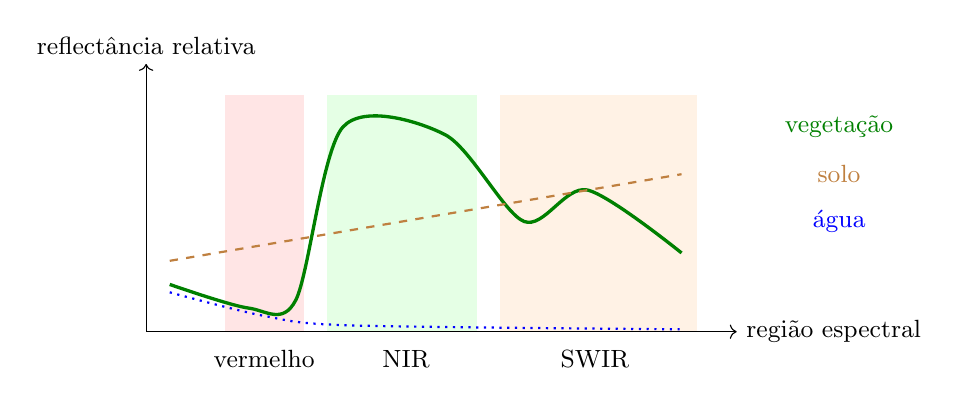
\begin{tikzpicture}[x=1cm,y=1cm,font=\small]
\fill[red!10] (1,0) rectangle (2,3);
\fill[green!10] (2.3,0) rectangle (4.2,3);
\fill[orange!10] (4.5,0) rectangle (7,3);
\draw[->] (0,0)--(7.5,0) node[right]{região espectral};
\draw[->] (0,0)--(0,3.4) node[above]{reflectância relativa};
\draw[very thick,green!50!black] plot[smooth] coordinates {(0.3,0.6)(1.3,0.3)(1.9,0.4)(2.5,2.6)(3.8,2.5)(4.8,1.4)(5.6,1.8)(6.8,1)};
\draw[thick,brown,dashed] (0.3,0.9)--(6.8,2);
\draw[thick,blue,dotted] plot[smooth] coordinates {(0.3,0.5)(1.5,0.2)(2.6,0.08)(6.8,0.03)};
\node at (1.5,-0.35){vermelho}; \node at (3.3,-0.35){NIR}; \node at (5.7,-0.35){SWIR};
\node[green!50!black] at (8.8,2.6){vegetação};
\node[brown] at (8.8,2){solo}; \node[blue] at (8.8,1.4){água};
\end{tikzpicture}
\caption{Comportamento espectral esquemático. Curvas qualitativas sem escala numérica, não medições. Fonte: elaborado pelo autor, síntese conceitual de \citet{WEISS2020}.}
\label{fig:espectro}
\end{figure*}
\begin{figure*}[htbp]
\centering\small
\begin{tabular}{lllll}
\hline Banda & Região & Centro S2A / S2B (nm) & Resolução & Índice no sistema\\ \hline
B4 & Vermelho & 664,5 / 665 & 10 m & NDVI\\
B8 & NIR amplo & 835,1 / 833 & 10 m & NDVI, NDWI\\
B8A & NIR estreito & 864,8 / 864 & 20 m & NDMI\\
B11 & SWIR & 1613,7 / 1610,4 & 20 m & NDWI, NDMI\\ \hline
\end{tabular}

\begin{tikzpicture}[x=0.009cm,y=0.6cm,font=\small]
\draw[->] (600,0)--(1730,0) node[right]{nm};
\foreach \x in {665,835,865,1614}{\draw[thick] (\x,0)--(\x,1);}
\node at (665,1.5){B4}; \node at (805,1.5){B8};
\node at (895,2){B8A}; \node at (1614,1.5){B11};
\end{tikzpicture}
\caption{Bandas dos índices. Centros espectrais por instrumento e resoluções nativas conforme o catálogo harmonizado \citep{GOOGLE_S2_SR}. Fonte: elaborado pelo autor.}
\label{fig:bandas}
\end{figure*}
\begin{figure*}[htbp]
\centering
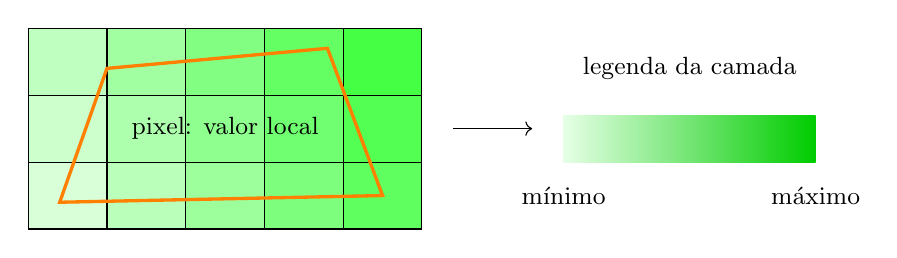
\begin{tikzpicture}[x=1cm,y=0.85cm,font=\small]
\foreach \x in {0,...,4}{\foreach \y in {0,...,2}{
\pgfmathtruncatemacro{\shade}{15+12*\x+5*\y}
\fill[green!\shade] (\x,\y) rectangle +(1,1);}}
\draw[step=1] (0,0) grid (5,3);
\draw[very thick,orange] (0.4,0.4)--(4.5,0.5)--(3.8,2.7)--(1,2.4)--cycle;
\node at (2.5,1.5){pixel: valor local};
\draw[->] (5.4,1.5)--(6.4,1.5);
\shade[left color=green!10,right color=green!80!black] (6.8,1) rectangle (10,1.7);
\node at (6.8,0.5){mínimo}; \node at (10,0.5){máximo};
\node at (8.4,2.4){legenda da camada};
\end{tikzpicture}
\caption{Polígono vetorial, células raster e gradiente em esquema sem dados reais. A geometria e as máscaras determinam o suporte válido. Fonte: elaborado pelo autor.}
\label{fig:raster-vetor}
\end{figure*}
\begin{figure*}[htbp]
\centering\small
\begin{tabular}{lcccl}
\hline & Pixel A & Pixel B & Média espacial & Operação\\ \hline
Aquisição 1 & 0,1 & 0,9 & 0,5 & média dos pixels\\
Aquisição 2 & 0,2 & 0,8 & 0,5 & média dos pixels\\
Aquisição 3 & 0,9 & 0,7 & 0,8 & média dos pixels\\ \hline
Mediana por pixel & 0,2 & 0,8 & 0,5 & média da composição\\ \hline
\end{tabular}
\caption{Ilustração matemática: a média das médias por aquisição é 0,6, enquanto a média da composição mediana é 0,5. Pesos iguais, sem máscaras; não é resultado experimental. Fonte: elaborado pelo autor.}
\label{fig:composicao}
\end{figure*}
\begin{figure*}[htbp]
\centering
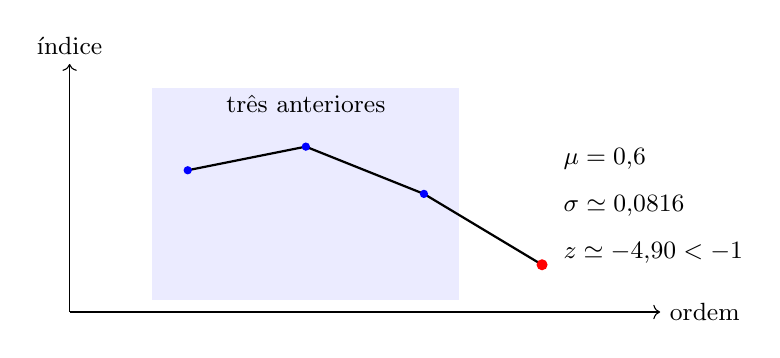
\begin{tikzpicture}[x=1.5cm,y=3cm,font=\small]
\fill[blue!8] (0.7,0.05) rectangle (3.3,0.95);
\draw[->] (0,0)--(5,0) node[right]{ordem};
\draw[->] (0,0)--(0,1.05) node[above]{índice};
\draw[thick] (1,0.6)--(2,0.7)--(3,0.5)--(4,0.2);
\foreach \x/\y in {1/0.6,2/0.7,3/0.5}{\fill[blue] (\x,\y) circle (1.5pt);}
\fill[red] (4,0.2) circle (2pt);
\node at (2,0.88){três anteriores};
\node[anchor=west] at (4.1,0.65){$\mu=0{,}6$};
\node[anchor=west] at (4.1,0.45){$\sigma\simeq0{,}0816$};
\node[anchor=west] at (4.1,0.25){$z\simeq-4{,}90<-1$};
\end{tikzpicture}
\caption{Janela e sinalização em sequência didática. Valores criados para ilustrar a regra, não observações agrícolas ou medida de eficácia. Fonte: elaborado pelo autor.}
\label{fig:janela}
\end{figure*}


\section{Trabalhos relacionados}\label{sec:relacionados-final}

O estudo de \citet{SLAIFFER2023} e sua publicação posterior \citep{SLAIFFER2025} investigam índices e produtividade da soja em áreas irrigadas e de sequeiro. Na publicação, mapas de produtividade da colhedora são relacionados a índices do Crop Monitoring por análises estatísticas e espaciais. Essa comparação evidencia uma diferença de objeto: enquanto o estudo investiga a relação entre indicadores e produtividade medida, este trabalho constrói o fluxo computacional que disponibiliza indicadores para exploração.

\citet{IZQUIERDO2026} integram sensores de campo, Sentinel-1, Sentinel-2 e dados agroclimáticos para modelar umidade em pomares de citros, com avaliação em anos independentes. A combinação de referência de campo e modelagem física e supervisionada permite avaliar estimativas de umidade. A plataforma aqui desenvolvida atua em outra etapa: organiza consulta, visualização e exportação de índices, sem treinamento de um estimador.

As revisões de \citet{WEISS2020} e \citet{PATRICIO2018} situam essas aplicações em um conjunto mais amplo de sensores e técnicas computacionais. Para este artefato, a questão central não é selecionar um modelo preditivo, mas coordenar representações, serviços e saídas de maneira verificável.

No monitoramento operacional, \citet{MERONI2019} examinam produtos MODIS utilizados pelo ASAP e pela autoridade de gestão de secas do Quênia. Seu tratamento de histórico sazonal, consolidação e erros mostra a importância da referência temporal para interpretar alertas. Em contraste, a regra deste sistema é exploratória e local à série; sua avaliação computacional não constitui avaliação de desempenho de um sistema de alerta agronômico.

No nível de infraestrutura, o Earth Engine oferece processamento programável, não substituindo a interface e os contratos desenvolvidos neste projeto \citep{GORELICK2017}. EOSDA Crop Monitoring e OneSoil são produtos finais. O guia oficial da EOSDA documenta desenho e importação de áreas, índices, gráficos, clima, leitura de valores por posição e downloads. Também diferencia recursos conforme plano e complementos \citep{EOSDA_GUIDE}. A página oficial da OneSoil documenta áreas, monitoramento espectral, comparação entre safras, clima e exportação de limites e mapas, distinguindo Mobile, Pro e assinaturas \citep{ONESOIL_PLATFORM_DETAIL}.

A \cref{tab:plataformas} apresenta uma comparação documental de funcionalidades, com fontes consultadas em novembro de 2026. EOSDA também oferece leitura por posição; a contribuição do artefato está na implementação documentada desse recurso e de seus contratos, não em sua exclusividade. A comparação não mede desempenho ou retorno financeiro.

\begin{table*}[htbp]
\centering\small
\caption{Comparação documental por finalidade e funcionalidades. As fontes oficiais dos produtos são \citet{EOSDA_GUIDE} e \citet{ONESOIL_PLATFORM_DETAIL}; Earth Engine é infraestrutura programável, não produto final equivalente. Recursos comerciais dependem de plano e modalidade.}
\label{tab:plataformas}
\setlength{\tabcolsep}{3pt}
\begin{tabular}{p{0.18\textwidth}p{0.18\textwidth}p{0.18\textwidth}p{0.18\textwidth}p{0.18\textwidth}}
\hline Critério & EOSDA & OneSoil & Earth Engine & Sistema\\ \hline
Natureza & Produto final & Produto final & Infraestrutura & Artefato acadêmico\\
Áreas & Desenho e importação & Desenho, seleção e upload & Geometrias por API & Desenho, nomes e GeoJSON\\
Exploração & Índices e gráficos por data & Monitoramento e comparação entre safras & Coleções e redutores & Composição e série por aquisição\\
Clima & Histórico e previsão & Clima e chuva & Integração por programação & Consulta diária NASA POWER\\
Saídas & Downloads documentados & Limites e mapas para máquinas & Exportação por programação & PDF, XLSX, CSV e GeoJSON\\
Acesso & Planos e complementos & Mobile/Pro e assinaturas & Projeto, elegibilidade e cotas & Web; cotas de serviços externos\\ \hline
\end{tabular}
\end{table*}

A distinção central é de finalidade: os produtos comerciais incluem gestão e recursos contratados; o Earth Engine oferece infraestrutura programável; e o artefato concentra um fluxo de seleção, processamento e exportação cuja implementação e verificação podem ser examinadas. Esse posicionamento permite discutir decisões de engenharia sem estabelecer superioridade funcional ou agronômica.

\section{Materiais e métodos}\label{chap:metodos-final}

\subsection{Caracterização da pesquisa e fontes de evidência}

O trabalho caracteriza-se como pesquisa aplicada e tecnológica em Ciência da Computação, cujo principal resultado é a plataforma desenvolvida. Sua construção e avaliação envolveram consulta à literatura, definição das funcionalidades, implementação em módulos e verificações do funcionamento. A avaliação se concentra no software, não em um experimento agronômico. O estudo bibliográfico não seguiu um protocolo de revisão sistemática, e não se atribui ao projeto a adoção formal de \textit{Design Science Research}, pois esse procedimento não foi documentado.

Para descrever o que foi efetivamente desenvolvido, a revisão tomou o código-fonte como referência principal, em vez de assumir que todos os itens previstos estavam implementados. Foram examinados os arquivos que iniciam a aplicação, os módulos Python, o componente HTML/JavaScript, as regras de armazenamento e exportação, o conjunto de testes, as especificações e os documentos acadêmicos. A proposta original foi tratada como registro do planejamento. A relação entre objetivos, requisitos, funções, testes e seções do artigo está organizada em \path{docs/artigo_final/RASTREABILIDADE_TCC.md}, distinguindo o que foi implementado do que foi avaliado.

O desenvolvimento foi organizado em especificações de funcionalidades e tarefas realizadas em branches, isto é, ramificações do controle de versão, com revisão das alterações antes da integração. O histórico registra entregas de interface, armazenamento e exportação acompanhadas por testes. Na correção dos contratos de dados, novos testes foram executados antes das mudanças para reproduzir as divergências e, depois, verificar se haviam sido corrigidas. Esse procedimento localizado não permite afirmar que todo o projeto seguiu desenvolvimento orientado a testes (TDD, \textit{Test-Driven Development}). O controle das dependências e a divisão de responsabilidades entre módulos apoiaram a evolução incremental; não foi identificada configuração de integração contínua no repositório.

\subsection{Materiais e ambiente}

A solução foi implementada em Python. O Streamlit coordena a interface e o estado da sessão, enquanto Folium/Leaflet apresentam os mapas e o Earth Engine executa as operações raster. Após a transferência dos resultados, NumPy e pandas organizam os dados locais e Plotly produz os gráficos. Para disponibilizar esses resultados fora da interface, ReportLab, Pillow e Matplotlib apoiam os relatórios estáticos, e openpyxl gera planilhas. A biblioteca geemap permanece em operações e mapas auxiliares, mas não é responsável por toda a interface atual.

O arquivo \texttt{requirements.txt} fixa dependências diretas e transitivas. A execução da suíte registrada nas evidências utilizou Linux x86\_64, Python 3.14.4, pytest 9.0.3, pytest-cov 7.1.0 e coverage 7.14.0. A identificação dessas versões situa o resultado dos testes, mas não demonstra reprodução em todos os sistemas operacionais ou na hospedagem. Os registros de preparação do Streamlit Community Cloud descrevem separadamente a resolução de dependências para Python 3.12.

\subsection{Entradas e requisitos}

As entradas principais são um polígono, duas datas e a escolha de NDVI, NDWI, NDMI ou todos os índices. A busca textual serve para navegação, não para inferir automaticamente limites de uma propriedade. A análise depende de geometria válida e intervalo cuja data final não anteceda a inicial. Salvar uma localização não executa análise nem associa automaticamente uma cultura.

O sistema permite selecionar a área, consultar imagens Sentinel-2, aplicar filtros, calcular índices e apresentar mapas, séries, sinalizações de anomalias e informações meteorológicas. Também permite nomear e reutilizar áreas e exportar resultados. Quanto às características de qualidade, a divisão em módulos pode ser examinada no código e a cobertura dos testes pode ser medida. Já a simplicidade da interface, o tempo de resposta inferior a 30 s, o baixo consumo e a redução de custos não foram demonstrados por avaliações específicas. Na execução local, a própria máquina precisa executar o servidor Streamlit, sem exigir um servidor dedicado separado.

\subsection{Aquisição de imagens e qualidade}

O módulo \texttt{earth\_engine.py} consulta a coleção \texttt{COPERNICUS/S2\_SR\_HARMONIZED} e mantém as imagens que possuem interseção com a área selecionada. Na interface, as datas inicial e final fazem parte do período solicitado, em Tempo Universal Coordenado (UTC). O Earth Engine, porém, não inclui o instante final de \texttt{ee.Filter.date}. Por isso, a aplicação envia o início do dia seguinte como limite: $[d_{\mathrm{inicial}},d_{\mathrm{final}}+1\ \mathrm{dia})$ \citep{GOOGLE_EE_DATE}. Assim, selecionar a mesma data nos dois campos corresponde a um dia completo. Uma data final anterior à inicial é rejeitada.

Antes de calcular os índices, o sistema filtra as imagens pela informação de cobertura de nuvens do produto. A condição padrão é estrita: \texttt{CLOUD\_COVERAGE\_ASSESSMENT < 20}, portanto o valor deve ser inferior a 20. Essa informação descreve o arquivo do produto que contém o grânulo, não uma medição de nuvens feita dentro da área selecionada. Todas as imagens aprovadas nos filtros seguem para o processamento; não é escolhida apenas a mais recente ou a menos nublada.

Depois desse filtro, a banda de qualidade QA60 é usada para excluir posições marcadas como nuvens opacas ou cirrus. A máscara mantém somente as posições em que os bits 10 e 11 dessa banda são zero. O conjunto selecionado contém B2, B3, B4, B8, B8A, B11 e QA60, embora B2 e B3 não entrem nas três equações dos índices.

Esse procedimento não inclui uma máscara adicional específica para sombras, neve ou probabilidade de nuvens. Há também uma restrição histórica: o catálogo informa que QA60 esteve mascarada entre 25/01/2022 e 28/02/2024, inclusive, e descreve sua posterior reconstrução a partir de classificações auxiliares \citep{GOOGLE_S2_SR}. Assim, encontrar imagens na coleção não garante que restarão dados úteis após aplicar a máscara em qualquer período.

Os índices das \cref{eq:ndvi-final,eq:ndwi-final,eq:ndmi-final} são calculados por \texttt{normalizedDifference}, renomeados e associados a \texttt{system:time\_start} e \texttt{system:index}. A série preserva data, valor e identificador de aquisição quando disponível, permitindo distinguir observações do mesmo dia.

\subsection{Produtos espaciais e temporais}\label{sec:agregacoes-final}

O processamento produz um mapa que combina o período e uma série que mantém os resultados de cada aquisição. Para formar o mapa, o sistema calcula primeiro o índice em cada imagem e depois combina seus valores por mediana em cada posição. Representando por $I_k(p,t)$ o índice $k$ na posição $p$ e aquisição $t$, após as máscaras, a composição é:
\begin{equation}\label{eq:composto-final}
 C_k(p)=\operatorname{mediana}_{t\in T_p} I_k(p,t),
\end{equation}
em que $T_p$ reúne as observações válidas naquela posição. A ordem é importante: calcula-se a mediana dos índices já obtidos, não o índice a partir de uma mediana prévia das bandas.

Para apresentar um único valor junto ao mapa, o sistema calcula a média espacial da composição $C_k$. Para construir a série temporal, calcula a média espacial separadamente em cada imagem. As duas operações usam o redutor de média do Earth Engine, mas recebem imagens diferentes. Elas podem ser representadas por:
\begin{align}
 M_k&=\frac{\sum_{p\in P_C}w_{p,C}C_k(p)}
                {\sum_{p\in P_C}w_{p,C}},\label{eq:media-composto}\\
 S_k(t)&=\frac{\sum_{p\in P_t}w_{p,t}I_k(p,t)}
                  {\sum_{p\in P_t}w_{p,t}}.\label{eq:serie-final}
\end{align}
Nessas expressões, $P_C$ e $P_t$ são os conjuntos de posições válidas, e $w$ indica quanto cada posição contribui para a média. A soma dos pesos, no denominador, deve ser positiva. No redutor ponderado padrão, o peso é o menor valor entre a máscara e a fração aproximada do pixel coberta pela área, não o produto dos dois. Essa fração é representada internamente em oito bits; interseções inferiores a aproximadamente $1/256$ podem receber peso zero \citep{GOOGLE_EE_REGION}.

A aplicação não acrescenta outra ponderação ao resultado. A chamada é \texttt{ee.Reducer.mean()}, com escala de processamento \texttt{scale=10} e limite \texttt{maxPixels=1e9}, sem definição explícita de \texttt{crs} nessa etapa \citep{GOOGLE_EE_REDUCE}.

Cada resultado responde a uma pergunta diferente. $C_k(p)$ informa o valor de uma posição no mapa composto; $M_k$ resume esse mapa em uma média da área; e $S_k(t)$ informa a média da área em uma aquisição. Esses valores não devem ser usados como se fossem equivalentes. Também é necessário considerar a grade espacial: o sistema de referência de coordenadas (CRS) não é fixado explicitamente nas reduções anteriores. A grade em projeção Universal Transversa de Mercator (UTM), com escala de 10 m, é definida depois, para a consulta interativa.

Ao organizar a série em \texttt{time\_series.py}, o sistema omite os registros sem valor retornado pelo serviço, converte os demais em números e os ordena pela data no formato ISO. Não estima valores entre as observações, não preenche lacunas e não faz agrupamento mensal ou composição diária. Imagens diferentes de uma mesma data podem gerar registros distintos, pois datas repetidas não são eliminadas. A contagem de imagens da coleção é feita antes da máscara; por isso, pode ser maior que a quantidade de pontos válidos na série.

\begin{figure*}[htbp]
\centering
\resizebox{0.96\textwidth}{!}{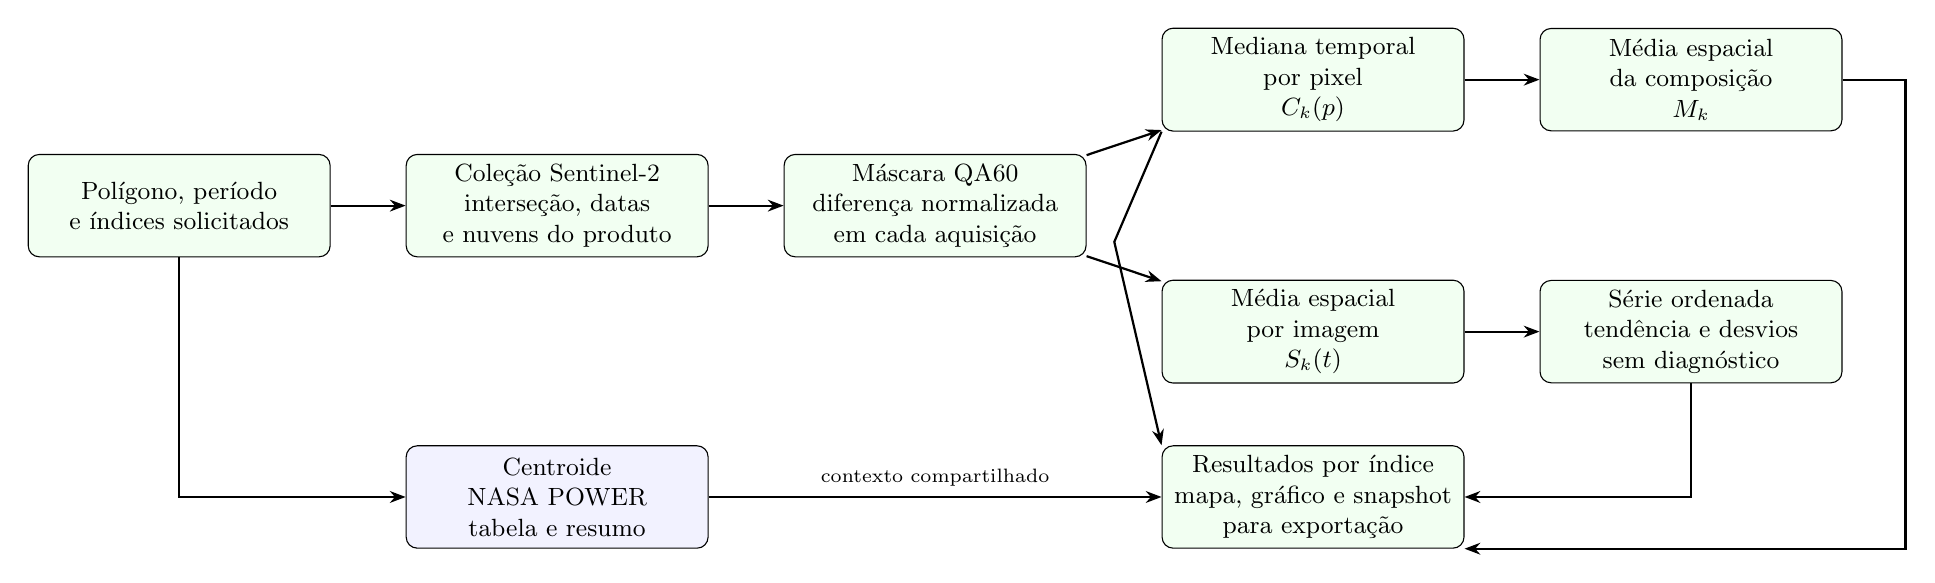
\begin{tikzpicture}[
 box/.style={draw,rounded corners,align=center,text width=36mm,
 minimum height=13mm,font=\small,fill=green!5},
 link/.style={-{Stealth[length=2mm]},thick}]
\node[box] (input) at (0,0) {Polígono, período\\e índices solicitados};
\node[box] (query) at (4.8,0) {Coleção Sentinel-2\\interseção, datas\\e nuvens do produto};
\node[box] (indices) at (9.6,0) {Máscara QA60\\diferença normalizada\\em cada aquisição};
\node[box] (spatial) at (14.4,1.6) {Mediana temporal\\por pixel\\$C_k(p)$};
\node[box] (mean) at (19.2,1.6) {Média espacial\\da composição\\$M_k$};
\node[box] (series) at (14.4,-1.6) {Média espacial\\por imagem\\$S_k(t)$};
\node[box] (anomaly) at (19.2,-1.6) {Série ordenada\\tendência e desvios\\sem diagnóstico};
\node[box,fill=blue!5] (climate) at (4.8,-3.7) {Centroide\\NASA POWER\\tabela e resumo};
\node[box] (output) at (14.4,-3.7) {Resultados por índice\\mapa, gráfico e snapshot\\para exportação};
\draw[link] (input) -- (query);
\draw[link] (query) -- (indices);
\draw[link] (indices) -- (spatial);
\draw[link] (spatial) -- (mean);
\draw[link] (indices) -- (series);
\draw[link] (series) -- (anomaly);
\draw[link] (input.south) |- (climate.west);
\draw[link] (climate) -- node[above,font=\scriptsize] {contexto compartilhado} (output);
\draw[link] (anomaly.south) |- (output.east);
\draw[link] (mean.east) -- ++(0.8,0) |- (output.south east);
\draw[link] (spatial.south west) -- ++(-0.6,-1.4) -- (output.north west);
\end{tikzpicture}
}
\caption{Derivação dos produtos espaciais e temporais a partir da coleção filtrada. Fonte: elaborado pelo autor a partir de \texttt{pipeline.py} e \texttt{time\_series.py}.}
\label{fig:fluxo-analise}
\end{figure*}

\subsection{Regra de detecção e tendência}\label{sec:anomalias-final}

Para sinalizar quedas na série, o sistema compara cada valor com os três registros imediatamente anteriores. Primeiro, calcula a média e o desvio padrão desses registros; depois, verifica quanto o valor atual se afasta dessa referência. Esse afastamento é expresso pelo escore $z_i$. A janela considera três observações, não três dias, pois o intervalo entre imagens pode variar. Nas equações seguintes, $x_i$ representa o valor na posição $i$ da série, com contagem iniciada em zero. O cálculo pode ser aplicado a partir da quarta observação, quando $i\geq3$:
\begin{align}
 \mu_i&=\frac{1}{3}\sum_{j=i-3}^{i-1}x_j,\\
 \sigma_i&=\sqrt{\frac{1}{3}\sum_{j=i-3}^{i-1}(x_j-\mu_i)^2},\\
 z_i&=\frac{x_i-\mu_i}{\sigma_i},\quad \sigma_i>0.\label{eq:escore-final}
\end{align}
O algoritmo marca anomalia somente quando $z_i<-1$: o valor atual deve estar mais de um desvio padrão abaixo da média dos três anteriores. Os três primeiros registros não têm uma janela completa e não são sinalizados. O mesmo ocorre quando $\sigma_i=0$, pois não é possível dividir o desvio por zero. Nesses casos, a saída armazena escore zero por convenção do algoritmo, não como resultado de um escore calculado.

O desvio padrão usa o divisor $N$, correspondente à opção \texttt{ddof=0} do NumPy, em vez de $N-1$ da fórmula amostral \citep{NUMPY_STD}. A denominação populacional dessa fórmula não significa que os três valores representem todas as condições agrícolas possíveis. A média usa apenas os registros anteriores e exclui o valor atual.

A função \texttt{detect\_anomalies} pressupõe entradas numéricas compatíveis, sem tratamento adicional específico de NaN, marcador de valor não numérico. Valores já sinalizados continuam participando das janelas seguintes. A janela de três registros e o limiar $-1$ são escolhas heurísticas, isto é, regras particulares da aplicação sem calibração experimental documentada. Elas não modelam sazonalidade nem são ajustadas por cultura.

Para resumir a tendência, o sistema ajusta uma reta à sequência de valores. A função \texttt{np.polyfit} calcula $x_i\simeq a\,i+b$ pelo método dos mínimos quadrados, minimizando $\sum_i[x_i-(a\,i+b)]^2$ \citep{HYNDMAN2021,NUMPY_POLYFIT}. O coeficiente $a$ é a inclinação, que indica a variação do índice por posição na sequência; $b$ é o intercepto, o valor da reta na posição zero.

A tendência é classificada como crescente se $a>0{,}01$, decrescente se $a<-0{,}01$ e estável nos demais casos. Esses limites também são heurísticos, sem calibração documentada. Como o ajuste usa a ordem das observações e não os dias transcorridos, a inclinação não é uma taxa diária. Quando há menos de dois pontos, a função retorna o rótulo estável por convenção, embora os dados sejam insuficientes para estimar uma inclinação.

\begin{figure*}[htbp]
\centering
\resizebox{0.92\textwidth}{!}{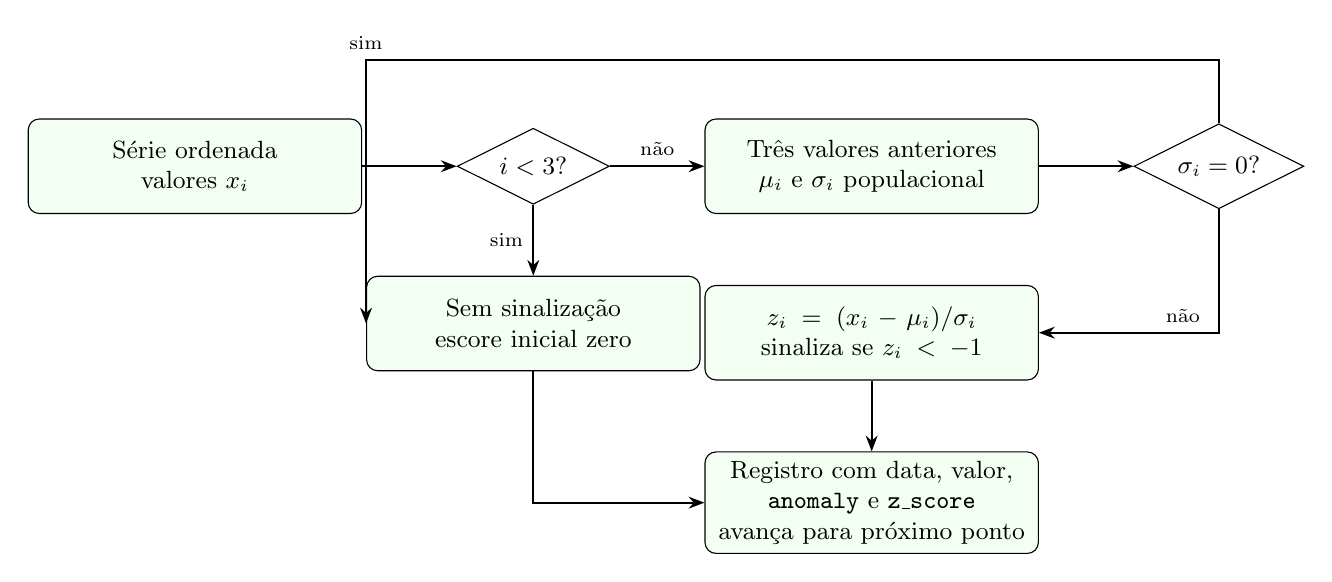
\begin{tikzpicture}[
 node distance=9mm and 12mm,
 box/.style={draw,rounded corners,align=center,text width=40mm,
 minimum height=12mm,font=\small,fill=green!5},
 decision/.style={draw,diamond,aspect=2,align=center,font=\small,inner sep=1mm},
 link/.style={-{Stealth[length=2mm]},thick}]
\node[box] (input) {Série ordenada\\valores $x_i$};
\node[decision,right=of input] (initial) {$i<3$?};
\node[box,right=of initial] (window) {Três valores anteriores\\$\mu_i$ e $\sigma_i$ populacional};
\node[decision,right=of window] (zero) {$\sigma_i=0$?};
\node[box,below=of window] (score) {$z_i=(x_i-\mu_i)/\sigma_i$\\sinaliza se $z_i<-1$};
\node[box,below=of initial] (false) {Sem sinalização\\escore inicial zero};
\node[box,below=of score] (output) {Registro com data, valor,\\\texttt{anomaly} e \texttt{z\_score}\\avança para próximo ponto};
\draw[link] (input)--(initial);
\draw[link] (initial)--node[above,font=\scriptsize]{não}(window);
\draw[link] (initial)--node[left,font=\scriptsize]{sim}(false);
\draw[link] (window)--(zero);
\draw[link] (zero.south)|-node[above,font=\scriptsize,pos=.6]{não}(score.east);
\draw[link] (zero.north)--++(0,0.8)-|node[above,font=\scriptsize,pos=.5]{sim}(false.west);
\draw[link] (false.south)|-(output.west);
\draw[link] (score)--(output);
\end{tikzpicture}
}
\caption{Heurística unilateral de sinalização de desvios negativos. Fonte: elaborado pelo autor a partir de \texttt{anomalies.py}.}
\label{fig:fluxo-anomalias}
\end{figure*}

\subsection{Consulta e agregação meteorológica}\label{sec:clima-final}

O contexto meteorológico é obtido por uma consulta diária da NASA POWER nas coordenadas do centroide calculado pelo Earth Engine. A requisição usa o serviço \texttt{/api/temporal/daily/point}, a comunidade agrícola \texttt{community=ag}, datas no formato \texttt{YYYYMMDD}, resposta JSON e tempo limite de 30 s. São solicitados os parâmetros \texttt{PRECTOTCORR}, \texttt{T2M} e \texttt{ALLSKY\_SFC\_SW\_DWN}. Embora o código contenha nomes internos para \texttt{T2M\_MAX} e \texttt{T2M\_MIN}, o fluxo padrão não consulta temperaturas máximas e mínimas.

No catálogo diário da comunidade agrícola, \texttt{PRECTOTCORR} corresponde à precipitação corrigida, em mm/dia; \texttt{T2M}, à temperatura média do ar a 2 m, em °C; e \texttt{ALLSKY\_SFC\_SW\_DWN}, à energia solar de ondas curtas incidente em superfície horizontal sob todas as condições de céu, em MJ/m²/dia \citep{NASA_POWER_PARAMETERS}. Para a integração efetiva, prevalece a unidade declarada em cada resposta, especialmente na radiação.

A resposta é organizada em uma tabela ordenada por data. O código $-999$, usado para indicar ausência de dado, não é tratado como uma medição. Para resumir o período, o sistema soma a precipitação e calcula as médias de temperatura e radiação, usando separadamente as observações válidas de cada variável. Esses conjuntos de dias são representados por $D_P$, $D_T$ e $D_R$:
\begin{align}
 P_{\mathrm{total}}&=\sum_{d\in D_P} P_d,\\
 \overline{T}&=\frac{1}{|D_T|}\sum_{d\in D_T}T_d,\\
 \overline{R}&=\frac{1}{|D_R|}\sum_{d\in D_R} f(u)R_d.\label{eq:radiacao-codigo}
\end{align}
Na \cref{eq:radiacao-codigo}, $f(u)=1$ para MJ/m²/dia e $f(u)=3{,}6$ para kWh/m²/dia, conforme a unidade declarada nos metadados. A conversão decorre de $1\ \mathrm{kWh}=1000\ \mathrm{J/s}\times3600\ \mathrm{s}=3{,}6\ \mathrm{MJ}$, pelas definições de watt e prefixos do SI \citep{BIPM_SI}. Unidade ausente ou desconhecida torna a radiação indisponível e gera aviso, sem inferência pela magnitude. Valores não finitos, booleanos, inválidos e a sentinela $-999$ são descartados. A coluna normalizada em MJ/m²/dia é compartilhada pelo resumo e pelas exportações.

A soma da precipitação disponível não assegura cobertura integral do intervalo caso haja lacunas. A requisição define \texttt{time-standard=UTC}, mantendo as duas datas inclusivas em correspondência ao período espectral \citep{NASA_POWER_DAILY}. A consulta é compartilhada entre os índices da mesma análise. A apresentação conjunta fornece contexto, sem calcular correlação ou atribuir causalidade.

\subsection{Procedimentos de avaliação técnica}\label{sec:avaliacao-final}

A avaliação procurou verificar tanto regras locais quanto a comunicação entre as partes da aplicação. Testes unitários examinaram regras específicas; testes de integração verificaram a troca de dados entre componentes; e testes de regressão verificaram a manutenção de comportamentos já corrigidos. Essa distinção de escopos, assim como a diferença entre executar código e verificar seu comportamento, é discutida por \citet{BENDER2020}. A referência não implica adoção dos processos internos do Google.

A interação com serviços externos e a navegação em navegador foram registradas separadamente. Essa separação é necessária porque substituir um serviço durante um teste permite controlar sua resposta, mas não demonstra que o fluxo completo funciona com o serviço real.

Foi reexecutada a suíte existente com tracer C e cobertura de ramificações. Os testes espectrais verificam seleção de bandas, filtros e chamadas usando substitutos da API, não a aritmética remota sobre imagens reais. Os testes de persistência usam arquivos temporários; os de exportação inspecionam formatos e valores controlados. Alguns testes Streamlit usam widgets reais com serviços substituídos. A cobertura Python não mede execução JavaScript no navegador.

Uma requisição pública curta à NASA POWER verificou metadados e datas em uma coordenada técnica, sem identificação de cultura. A resposta histórica está em tempo solar local (LST, \textit{Local Solar Time}); foi preservada para reproduzir a divergência de unidade, não como evidência de uma nova consulta UTC. Seus valores foram reutilizados em testes de regressão de resumo e exportação. O componente JavaScript recebeu testes independentes de legenda, consulta e descompressão, e matrizes controladas permitiram medir o empacotamento de dados. Essas medições não foram usadas para inferir desempenho em produção.

\subsection{Avaliação com potenciais usuários}\label{sec:pesquisa-usuarios}

A avaliação com usuários buscou conhecer as tarefas que os respondentes disseram ter realizado, sua experiência de uso e a utilidade atribuída aos recursos. Trata-se de uma avaliação exploratória e descritiva, com análise quantitativa e qualitativa, não de uma verificação da eficácia agronômica da plataforma. Conforme informação do autor, o formulário \url{https://forms.gle/VXqtdCgH9us774VE6} foi divulgado por WhatsApp e LinkedIn para profissionais e estudantes de agronomia, produção rural, tecnologia e áreas afins.

Como cada pessoa decidiu participar voluntariamente, a coleta caracteriza amostragem não probabilística por adesão, sujeita à autoseleção \citep{AAPOR2013}. Não há um cadastro do público convidado que permita calcular a taxa de resposta ou afirmar representatividade populacional.

A apresentação solicita exploração prévia da plataforma, estima de 5 a 8 minutos para responder e orienta evitar informações pessoais. A planilha fornecida pelo autor contém uma aba de respostas com 50 colunas, incluindo o carimbo, a triagem e os itens de matrizes expandidos, e outra aba vazia. Foram identificados três itens de perfil, nove atividades, nove afirmações sobre uso, onze recursos avaliados quanto à utilidade, oito afirmações sobre compreensão e aplicabilidade, cinco campos discursivos e uma nota geral de 0 a 10. O conhecimento declarado refere-se à agricultura de precisão, não a uma medida direta de domínio de sensoriamento remoto; a experiência prévia e sua frequência são captadas em um mesmo item.

Antes dos cálculos, as respostas foram conferidas quanto à elegibilidade, ao preenchimento e à duplicidade. Os 31 registros indicam ``Sim'' na pergunta conjunta sobre maioridade, leitura e consentimento, e na declaração de exploração de ao menos um recurso. Não há duplicatas exatas, nem respostas integralmente iguais ao desconsiderar o carimbo. Não foram coletados identificadores individuais, e a unidade da análise descritiva é a submissão elegível ao questionário.

O conjunto analisado abrange respostas registradas entre 06 e 15 de novembro de 2026.

Nas tarefas, as categorias são ``Consegui sem ajuda'', ``Consegui com ajuda'', ``Tentei, mas não consegui'' e ``Não tentei''. A conclusão entre tentativas é a razão entre as duas primeiras e o total das três primeiras. O questionário agrega séries temporais e possíveis anomalias em uma atividade e reúne a exportação de relatório ou dados em outra; não se estimam taxas separadas para recursos que o instrumento não separou. Trata-se de autorrelato, sem observação controlada, cronometração ou inspeção dos logs de cada utilização.

As perguntas de concordância usam cinco categorias, de discordo totalmente a concordo totalmente. Nas perguntas de utilidade, as categorias vão de nada útil a muito útil; ``Moderadamente útil'' ocupa a posição intermediária, mas não significa neutralidade. Para respeitar essa ordenação, a análise prioriza a contagem e o percentual das respostas em cada categoria, a mediana e os quartis, conforme as cautelas discutidas por \citet{SULLIVAN2013}. Os agrupamentos 4--5, 3 e 1--2 ajudam a resumir os resultados sem substituir as distribuições completas.

A base de cálculo depende da pergunta. ``Não consegui avaliar'', ausências e valores inválidos são contados separadamente e não entram no total de respostas usado para os percentuais ordinais. Nas tarefas, ``Não tentei'' permanece na distribuição geral, mas fica fora do cálculo de conclusão entre tentativas. Não há preenchimento estimado de respostas ausentes.

Os quartis usam interpolação linear, e o intervalo interquartil é $Q_3-Q_1$. Médias e desvios padrão amostrais dos códigos ordinais são disponibilizados somente como descrições complementares; a nota geral recebe também moda, extremos e distribuição. Não se construíram escores agregados de usabilidade ou aceitação, nem se denominou o instrumento SUS, TAM, UTAUT ou NPS. Seis cruzamentos descritivos usam agrupamentos amplos, com supressão de grupos com menos de cinco respostas válidas, sem testes de hipótese ou conclusões causais. Isso reduz a exposição de pequenos grupos, mas não certifica anonimato.

As respostas abertas foram lidas integralmente e organizadas por temas, em diálogo com a referência de análise temática de \citet{BRAUN2006}. Foram identificados trechos com significado relevante, atribuídas categorias conforme seu conteúdo e revistos os agrupamentos. Uma resposta podia receber mais de uma categoria. Cada registro, porém, conta apenas uma vez em cada tema, mesmo quando o menciona em perguntas diferentes.

Foram codificadas 142 células preenchidas, e treze comentários opcionais estavam ausentes. O campo sobre impedimento de acesso estava vazio nos 31 registros; essa ausência foi considerada compatível com a triagem do formulário, não uma medição de dificuldade igual a zero. A codificação teve assistência de IA, e seus critérios e trechos literais sem identificação permanecem disponíveis para validação do autor. Não houve codificação independente por dois avaliadores nem medição de concordância entre eles.

A coleta utiliza a versão pública anterior às correções de radiação, legenda, clima multiíndice, intervalos, invalidação e IDs de aquisição. Por decisão do autor, essa versão foi mantida durante a coleta, sem implantação das alterações locais. As percepções dos respondentes não são atribuídas à versão aprimorada, consolidada no commit \texttt{28759bf}. A documentação da análise distingue essas versões; o commit exato da versão pública permanece pendente. A confirmação dos procedimentos éticos institucionais cabe ao autor e ao orientador; não se atribui aprovação ou dispensa formal sem documento.

\section{Desenvolvimento e implementação}\label{chap:implementacao-final}

\subsection{Arquitetura e divisão de responsabilidades}

A plataforma é uma aplicação modular executada em um processo Python com interface web, complementada por um componente JavaScript no navegador e serviços externos. A separação lógica entre apresentação, orquestração e acesso a dados não corresponde a microsserviços próprios ou a um backend REST independente. O Streamlit gerencia o ciclo de renderização e o estado da sessão.

O ponto de entrada local é \texttt{src/app/main.py}; o ponto de entrada web é \texttt{streamlit\_app.py}. Este último ajusta o caminho de importação, força armazenamento por sessão e autenticação por conta de serviço, carrega as configurações disponíveis nos Secrets e encaminha a execução à mesma função principal. A conta de serviço autentica a aplicação perante o Earth Engine, não o visitante \citep{GOOGLE_EE_SERVICE_ACCOUNT,STREAMLIT_CLOUD_SECRETS}.

\begin{figure*}[htbp]
\centering
\resizebox{0.96\textwidth}{!}{% Diagrama baseado em src/app e nas integrações observadas no código.
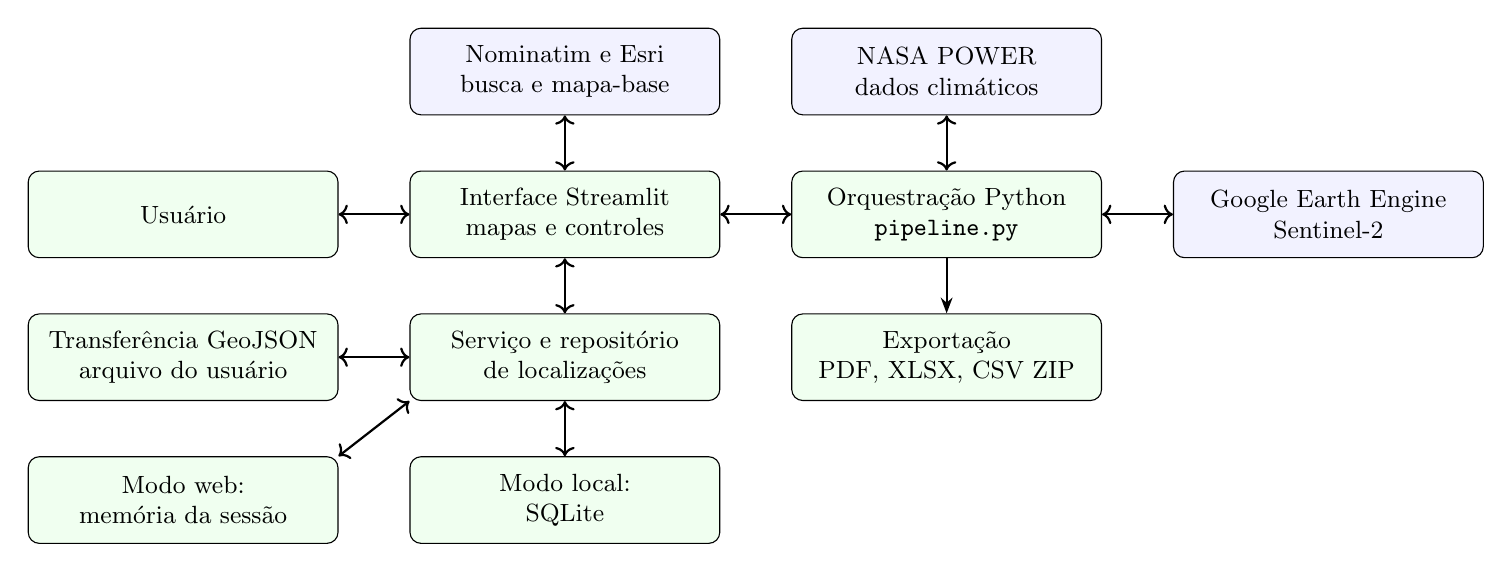
\begin{tikzpicture}[
  node distance=7mm and 9mm,
  box/.style={draw, rounded corners, align=center, minimum height=11mm,
    text width=37mm, font=\small, fill=green!6},
  external/.style={box, fill=blue!5},
  link/.style={-{Stealth[length=2mm]}, thick}
]
\node[box] (user) {Usuário};
\node[box, right=of user] (ui) {Interface Streamlit\\mapas e controles};
\node[box, right=of ui] (pipeline) {Orquestração Python\\\texttt{pipeline.py}};
\node[external, right=of pipeline] (gee) {Google Earth Engine\\Sentinel-2};
\node[external, above=of pipeline] (climate) {NASA POWER\\dados climáticos};
\node[external, above=of ui] (map) {Nominatim e Esri\\busca e mapa-base};
\node[box, below=of ui] (location) {Serviço e repositório\\de localizações};
\node[box, below=of pipeline] (export) {Exportação\\PDF, XLSX, CSV ZIP};
\node[box, below=of location] (sqlite) {Modo local:\\SQLite};
\node[box, left=of sqlite] (session) {Modo web:\\memória da sessão};
\node[box, left=of location] (geojson) {Transferência GeoJSON\\arquivo do usuário};
\draw[link,<->] (user) -- (ui);
\draw[link,<->] (ui) -- (pipeline);
\draw[link,<->] (pipeline) -- (gee);
\draw[link,<->] (pipeline.north) -- (climate.south);
\draw[link,<->] (ui.south) -- (location.north);
\draw[link,<->] (location.south) -- (sqlite.north);
\draw[link,<->] (location.south west) -- (session.north east);
\draw[link,<->] (geojson.east) -- (location.west);
\draw[link] (pipeline.south) -- (export.north);
\draw[link,<->] (ui.north) -- (map.south);
\end{tikzpicture}
}
\caption{Arquitetura implementada, com processamento no servidor Python, interação no navegador e serviços externos. Fonte: elaborado pelo autor a partir dos módulos do sistema.}
\label{fig:arquitetura-atual}
\end{figure*}

\begin{table*}[htbp]
\centering\small
\caption{Responsabilidades dos principais componentes implementados.}
\label{tab:componentes-final}
\begin{tabular}{p{0.25\textwidth}p{0.66\textwidth}}
\hline
\textbf{Componente} & \textbf{Responsabilidade e fronteira} \\ \hline
\texttt{main.py}, estilos & Controles, estado, validação de requisições, apresentação e ações de exportação. \\
\texttt{maps.py} & Geocodificação, mapas de seleção, conversão de geometrias, métricas, tiles e pré-carregamento de grades. \\
\texttt{map\_interaction.py}, HTML & Ponte Streamlit e mapa Leaflet com consulta local de valores raster. \\
\texttt{pipeline.py} & Coordenação da coleção, produtos por índice e contexto meteorológico. \\
\texttt{earth\_engine.py}, \texttt{time\_series.py} & Filtros, máscara, índices e redução espacial por aquisição. \\
\texttt{anomalies.py}, \texttt{climate.py} & Heurística temporal, tendência, requisições climáticas, tabela, gráfico e resumo. \\
Serviço e repositórios de localizações & Validação e operações de armazenamento SQLite ou em memória de sessão. \\
\texttt{export\_context.py}, exportadores & Snapshot normalizado e serialização em PDF, XLSX e CSV ZIP. \\ \hline
\end{tabular}
\end{table*}

O desenvolvimento incremental ampliou o núcleo de mapas e séries com análise multiíndice, exportações e armazenamento intercambiável. A implementação avaliada parte da revisão \texttt{b7c325c}, acrescida das correções de contratos e testes descritas na avaliação técnica.

\subsection{Busca geográfica e mapa de seleção}

A busca usa o endpoint público Nominatim \texttt{/search}, com texto normalizado, formato \texttt{jsonv2}, limite de um resultado e tempo limite de 10 s. O retorno contém descrição, latitude, longitude e caixa delimitadora. O zoom é estimado pela extensão dessa caixa e limitado de 1 a 20. A primeira resposta não comprova a identificação de uma propriedade rural; sua função é aproximar a navegação da região desejada.

O mapa de seleção é construído com Folium, tiles Esri World Imagery e ferramenta de polígono do Leaflet Draw. São habilitadas edição e remoção de desenhos. A análise utiliza uma área ativa obtida do evento de desenho; a existência de múltiplos desenhos no componente não implementa comparação automática entre talhões.

A conversão para \texttt{ee.Geometry.Polygon} verifica tipo, fechamento, coordenadas finitas, limites geográficos, quantidade de vértices e área planar não nula. Nesse caminho também são rejeitadas interseções próprias estritas entre segmentos não adjacentes. Isso não equivale a um validador topológico completo de polígonos, relações entre anéis e todos os casos degenerados. Área, perímetro e centroide analíticos são obtidos pelo Earth Engine e convertidos para hectares, quilômetros e coordenadas.

\subsection{Estado da interface e coerência entre entradas e saídas}

O estado distingue área ativa, parâmetros de análise, resultados por índice, grade de valores, URLs de tiles, snapshot e arquivos preparados. A inicialização evita sobrescrever valores em cada reexecução. O processamento apresenta estados de espera, execução, sucesso, ausência de imagens e erro. Falhas de autenticação impedem a continuidade da interface principal; falhas de clima são tratadas como indisponibilidade complementar pelo pipeline.

A aceitação de desenho, troca de área e busca bem-sucedida invalidam resultados associados à seleção anterior. A busca sem resultado preserva a seleção existente. A restauração de uma área é concluída somente após validação e obtenção das métricas; não chama o geocodificador nem inicia análise automática. Chaves de revisão do mapa e controle de eventos repetidos evitam reaplicar um polígono excluído ou perder desenhos durante reexecuções.

A alteração de geometria, período ou conjunto solicitado de índices invalida resultados, metadados, grades, tiles, snapshot e arquivos preparados. A alternância visual entre índices já calculados preserva esses produtos e não inicia consulta remota. A exportação também confere o snapshot antes da geração, aplicando a mesma preocupação de coerência entre entradas e saídas em uma fronteira adicional.

\subsection{Gerenciamento de localizações}

O serviço \texttt{SavedLocationsService} recebe nome e GeoJSON, aplica validações e coordena repositórios intercambiáveis. O registro contém identificador UUID, nome exibido, chave normalizada de comparação, geometria, coordenadas de enquadramento e datas UTC de criação e atualização. O nome é limitado a 100 caracteres; espaços são normalizados e a comparação utiliza \texttt{casefold}, sem distinguir caixa.

As coordenadas \texttt{center\_lat} e \texttt{center\_lon} persistidas correspondem ao ponto médio da caixa delimitadora, não ao centroide geométrico calculado no Earth Engine. A recuperação utiliza esse tipo de enquadramento para navegação, mas recalcula as métricas analíticas da área. Essa distinção evita confundir um centro de visualização com a coordenada da consulta climática.

No modo SQLite, uma tabela \texttt{saved\_locations} mantém GeoJSON serializado em texto, nomes e metadados. O caminho é configurável por \texttt{SAVED\_LOCATIONS\_DB\_PATH}; o padrão utiliza o diretório de dados do usuário. A inicialização é idempotente, usa \texttt{PRAGMA user\_version=1} e rejeita esquema futuro incompatível. Consultas parametrizadas, unicidade do nome normalizado e transações protegem o contrato de gravação. O armazenamento é da instância local e não oferece isolamento autenticado por pessoa.

No modo web, o repositório recebe um dicionário da sessão Streamlit e retorna cópias independentes. Não utiliza banco externo nem promete recuperação após encerramento ou perda da sessão. O limite do conjunto é verificado para que as localizações possam ser transferidas em um arquivo aceito pelo importador.

\begin{figure*}[htbp]
\centering
\resizebox{0.95\textwidth}{!}{% Recorte das classes reais de gerenciamento de localizações.
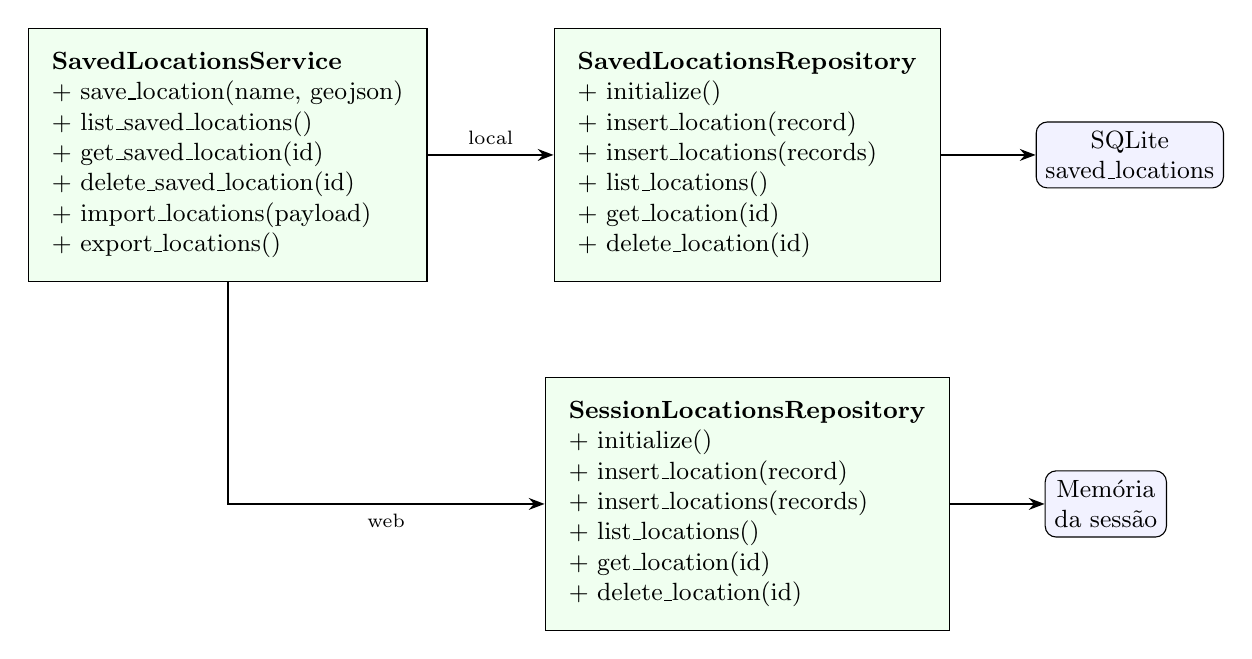
\begin{tikzpicture}[
  class/.style={draw, align=left, inner sep=3mm, font=\small, fill=green!6},
  link/.style={-{Stealth[length=2mm]}, thick}
]
\node[class] (service) at (0,0) {\textbf{SavedLocationsService}\\
  + save\_location(name, geojson)\\
  + list\_saved\_locations()\\
  + get\_saved\_location(id)\\
  + delete\_saved\_location(id)\\
  + import\_locations(payload)\\
  + export\_locations()};
\node[class, right=16mm of service] (repo) {\textbf{SavedLocationsRepository}\\
  + initialize()\\
  + insert\_location(record)\\
  + insert\_locations(records)\\
  + list\_locations()\\
  + get\_location(id)\\
  + delete\_location(id)};
\node[draw, rounded corners, align=center, right=12mm of repo,
  font=\small, fill=blue!5] (db) {SQLite\\saved\_locations};
\node[class, below=12mm of repo] (session) {\textbf{SessionLocationsRepository}\\
  + initialize()\\
  + insert\_location(record)\\
  + insert\_locations(records)\\
  + list\_locations()\\
  + get\_location(id)\\
  + delete\_location(id)};
\node[draw, rounded corners, align=center, right=12mm of session,
  font=\small, fill=blue!5] (memory) {Memória\\da sessão};
\draw[link] (service) -- node[above, font=\scriptsize] {local} (repo);
\draw[link] (service.south) |- node[below, font=\scriptsize, pos=0.75] {web} (session.west);
\draw[link] (repo) -- (db);
\draw[link] (session) -- (memory);
\end{tikzpicture}
}
\caption{Serviço e alternativas de armazenamento de localizações. Fonte: elaborado pelo autor a partir das classes implementadas.}
\label{fig:classes-localizacao}
\end{figure*}

A transferência aceita uma \texttt{Feature} ou \texttt{FeatureCollection}, contendo geometrias Polygon e nome em \texttt{properties.name}, limitada a 100 áreas e $2\times1024^2$ bytes. A importação valida o lote e rejeita duplicatas sem sobrescrever registros. No SQLite, a inserção é transacional; na sessão, a atualização ocorre após as verificações. IDs e datas são gerados novamente, não copiados do arquivo.

Há operações de exclusão no serviço e nos repositórios, porém não há ação correspondente na interface atual nem fluxo de renomeação. Também não são persistidos histórico de análises, credenciais ou objetos Earth Engine. A validação local de geometrias salvas verifica estrutura e área assinada de cada anel, mas não repete todos os testes de interseção do caminho de análise; as camadas não devem ser descritas como validadores topológicos equivalentes.

\begin{figure*}[htbp]
\centering
\resizebox{0.95\textwidth}{!}{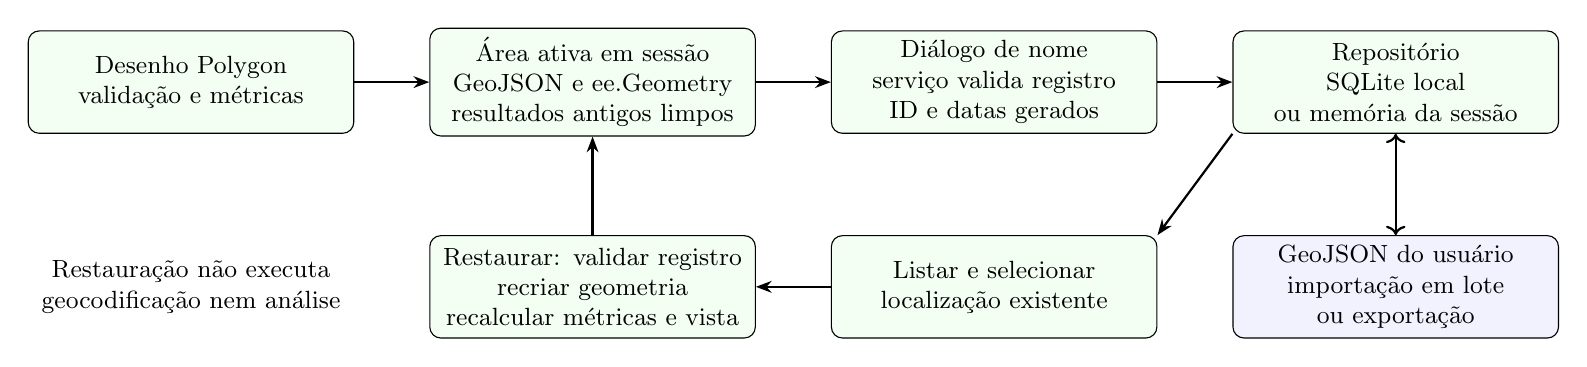
\begin{tikzpicture}[
 box/.style={draw,rounded corners,align=center,text width=39mm,
 minimum height=13mm,font=\small,fill=green!5},
 link/.style={-{Stealth[length=2mm]},thick}]
\node[box] (draw) at (0,0) {Desenho Polygon\\validação e métricas};
\node[box] (active) at (5.1,0) {Área ativa em sessão\\GeoJSON e ee.Geometry\\resultados antigos limpos};
\node[box] (save) at (10.2,0) {Diálogo de nome\\serviço valida registro\\ID e datas gerados};
\node[box] (storage) at (15.3,0) {Repositório\\SQLite local\\ou memória da sessão};
\node[box] (restore) at (5.1,-2.6) {Restaurar: validar registro\\recriar geometria\\recalcular métricas e vista};
\node[box] (list) at (10.2,-2.6) {Listar e selecionar\\localização existente};
\node[box,fill=blue!5] (file) at (15.3,-2.6) {GeoJSON do usuário\\importação em lote\\ou exportação};
\draw[link] (draw)--(active);
\draw[link] (active)--(save);
\draw[link] (save)--(storage);
\draw[link] (storage.south west)--(list.north east);
\draw[link] (list)--(restore);
\draw[link] (restore)--(active);
\draw[link,<->] (storage)--(file);
\node[font=\small,align=center] at (0,-2.6) {Restauração não executa\\geocodificação nem análise};
\end{tikzpicture}
}
\caption{Demarcação, gravação e restauração da área ativa, com alternativas de armazenamento. Fonte: elaborado pelo autor a partir da interface e do serviço de localizações.}
\label{fig:fluxo-areas}
\end{figure*}

\subsection{Orquestração e análise multiíndice}

Os caminhos individual e multiíndice compartilham consulta de coleção e métodos de cálculo. A versão multiíndice busca a coleção, aplica a máscara e obtém o clima compartilhado antes de produzir os resultados de cada índice. Os nomes repetidos são removidos preservando ordem. O pipeline não executa treinamento, classificação de culturas ou diagnóstico causal.

Os objetos de imagem permanecem referências a operações Earth Engine, enquanto estatísticas e séries são transferidas ao Python. A redução de cada aquisição é recuperada por chamadas individuais em uma iteração; essa estratégia simplifica a estrutura de retorno, mas pode aumentar latência e quantidade de requisições. Não há fila de tarefas, processamento distribuído próprio ou mecanismo de retomada persistente de uma análise interrompida.

\subsection{Pré-carregamento e consulta interativa}\label{sec:hover-final}

A exploração espacial utiliza dois produtos relacionados, mas distintos: tiles coloridos para renderização e uma grade numérica para consulta. Após o processamento, \texttt{preload\_index\_values} escolhe a zona UTM pelo centro informado e cria projeção norte ou sul em escala nominal de 10 m. Cada composição é selecionada, reprojetada, recortada pelo polígono e convertida em ponto flutuante. Bandas \texttt{grid\_x} e \texttt{grid\_y} permitem localizar a origem dos índices da grade.

A extração usa \texttt{sampleRectangle}, que retorna uma matriz por banda na projeção de entrada \citep{GOOGLE_EE_SAMPLE}. A região é a caixa delimitadora projetada da área; valores mascarados recebem $-9999$. O código estima a quantidade de células considerando também duas bandas de coordenadas e recusa estimativas superiores a dois milhões de valores. Uma verificação posterior confere a dimensão efetivamente recebida dos índices. Esse limite é do cliente da aplicação, não garantia de que o serviço remoto aceitará qualquer requisição abaixo dele.

As matrizes são convertidas para \texttt{float32} little-endian, comprimidas com zlib e codificadas em Base64. O componente recebe CRS, transformação afim, primeira linha/coluna, dimensões, sentinela e valores. No navegador, \texttt{DecompressionStream("deflate")} recupera os bytes e \texttt{Float32Array} permite acesso por posição. A compatibilidade desses recursos e das bibliotecas carregadas por CDN é requisito de execução, ainda não avaliado em uma matriz de navegadores.

Os eventos de movimento e toque verificam pertencimento ao polígono por teste de cruzamentos, incluindo exclusão de anéis internos. O componente projeta longitude/latitude em UTM com Proj4 e usa os termos de escala e origem da transformação. Para uma grade sem rotação, a localização é:
\begin{align}
 c&=\left\lfloor\frac{x-x_0}{s_x}\right\rfloor-c_0,\\
 r&=\left\lfloor\frac{y-y_0}{s_y}\right\rfloor-r_0,\qquad q=r\,n_c+c.
\end{align}
O índice linear $q$ acessa a matriz do indicador ativo. Termos de rotação/cisalhamento não são utilizados pelo JavaScript; o procedimento pressupõe a grade alinhada construída na etapa anterior. Fora do polígono, fora da matriz, com valor não finito ou com a sentinela, são exibidas mensagens específicas. Valores válidos aparecem com quatro casas decimais.

Não ocorre chamada ao Earth Engine a cada movimento do cursor. A interação consulta a grade já transferida; os tiles de fundo e da camada temática ainda dependem de carregamento de rede. O valor consultado representa a célula reamostrada da composição mediana do período, não uma leitura instantânea de campo, uma aquisição individual, a média temporal ou a média espacial de toda a área.

Uma medição reproduzível de empacotamento utilizou três matrizes controladas de $128\times128$ células, cada uma com 65.536 bytes em float32. Os tamanhos zlib foram 89 bytes para a matriz constante, 845 para o gradiente repetido e 60.562 para valores pseudoaleatórios com semente 42; em Base64, resultaram 120, 1.128 e 80.752 bytes. O contraste mostra que compressibilidade depende dos dados e que Base64 acrescenta volume. Não foram medidos tráfego total, latência de produção ou número observado de chamadas evitadas; arquiteturalmente, o lookup não solicita valores remotos por evento.

\begin{figure*}[htbp]
\centering
\resizebox{0.96\textwidth}{!}{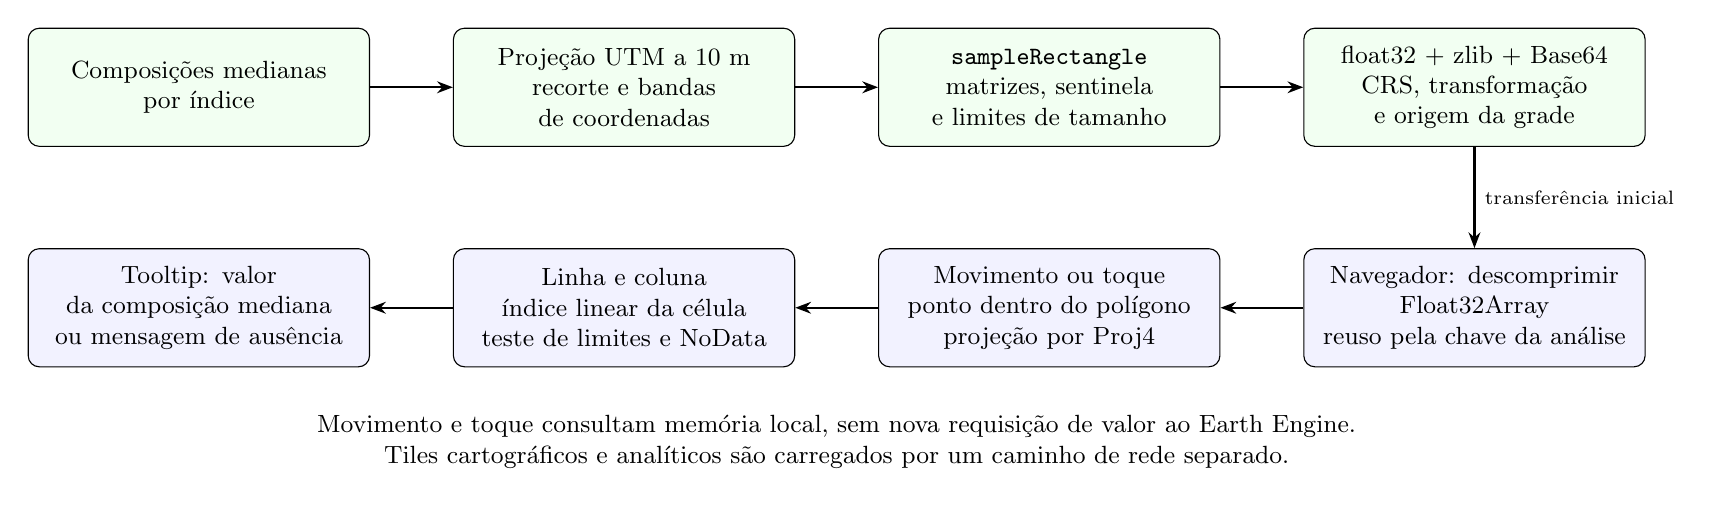
\begin{tikzpicture}[
 box/.style={draw,rounded corners,align=center,text width=41mm,
 minimum height=15mm,font=\small,fill=green!5},
 link/.style={-{Stealth[length=2mm]},thick}]
\node[box] (median) at (0,0) {Composições medianas\\por índice};
\node[box] (project) at (5.4,0) {Projeção UTM a 10 m\\recorte e bandas\\de coordenadas};
\node[box] (sample) at (10.8,0) {\texttt{sampleRectangle}\\matrizes, sentinela\\e limites de tamanho};
\node[box] (pack) at (16.2,0) {float32 + zlib + Base64\\CRS, transformação\\e origem da grade};
\node[box,fill=blue!5] (decode) at (16.2,-2.8) {Navegador: descomprimir\\Float32Array\\reuso pela chave da análise};
\node[box,fill=blue!5] (mouse) at (10.8,-2.8) {Movimento ou toque\\ponto dentro do polígono\\projeção por Proj4};
\node[box,fill=blue!5] (lookup) at (5.4,-2.8) {Linha e coluna\\índice linear da célula\\teste de limites e NoData};
\node[box,fill=blue!5] (tooltip) at (0,-2.8) {Tooltip: valor\\da composição mediana\\ou mensagem de ausência};
\draw[link] (median)--(project);
\draw[link] (project)--(sample);
\draw[link] (sample)--(pack);
\draw[link] (pack)--node[right,font=\scriptsize]{transferência inicial}(decode);
\draw[link] (decode)--(mouse);
\draw[link] (mouse)--(lookup);
\draw[link] (lookup)--(tooltip);
\node[font=\small,align=center] at (8.1,-4.5) {Movimento e toque consultam memória local, sem nova requisição de valor ao Earth Engine.\\Tiles cartográficos e analíticos são carregados por um caminho de rede separado.};
\end{tikzpicture}
}
\caption{Transferência da grade e consulta local por posição no navegador. Fonte: elaborado pelo autor a partir de \texttt{maps.py} e \texttt{index\_hover/index.html}.}
\label{fig:fluxo-consulta-pixel}
\end{figure*}

\subsection{Cores, legendas e mapas estáticos}

As paletas são sequenciais: branco--verde no NDVI, branco--azul no NDWI e tons claros--alaranjados--marrons no NDMI. No caminho interativo principal, os extremos são obtidos dos valores válidos da grade. Intervalos constantes recebem pequena expansão e conjuntos sem valores válidos usam $[-1,1]$. Os tiles são recortados pela geometria e obtidos com \texttt{getMapId}; a opacidade no Leaflet é 0,7.

A ponte Python transmite ao argumento \texttt{range} os mesmos extremos utilizados nos tiles. O navegador calcula mínimo, ponto médio e máximo da legenda a partir desse contrato, inclusive em intervalos negativos. Expansão de intervalos constantes e fallback sem dados são definidos antes da renderização, evitando escalas independentes entre camada e legenda.

No PDF, o renderizador estático usa intervalo fixo $[-1,1]$, thumbnail Earth Engine em EPSG:3857 e mosaico de tiles Esri. O contorno, gradiente e atribuição são desenhados com Pillow. Portanto, o PDF não é uma captura do componente interativo e pode ter contraste visual diferente. Falhas de rede ou renderização produzem estado explícito de mapa indisponível.

\subsection{Exportação e interoperabilidade}\label{sec:exportacao-final}

O snapshot concluído associa resultados à geometria e ao período. Antes de gerar um arquivo, a interface exige correspondência com os parâmetros atuais; o construtor normaliza datas e copia estruturas mutáveis, mantendo referências opacas a imagens e objetos gráficos. Não se realiza nova análise espectral para cada formato.

O PDF é gerado em memória com ReportLab em A4 paisagem, com uma página por índice presente no contexto, na ordem fornecida. Com os três índices, resulta em três páginas; com apenas um, em uma. Cada página reúne período, área, data de geração, média espacial da composição, tendência quando disponível, contagem de imagens quando fornecida, resumo meteorológico, série, anomalias e mapa estático. O nome da localização salva e coordenadas explícitas não são impressos automaticamente como identificação de propriedade. A lista de anomalias é resumida, exibindo até três ocorrências e indicação de excedentes. O PDF não substitui a saída tabular completa.

O XLSX contém \texttt{Resumo}, uma aba por índice selecionado, \texttt{Clima}, \texttt{Anomalias} e \texttt{Geografia}; são sete abas quando os três índices estão presentes. Nas abas espectrais, as colunas são \texttt{date}, \texttt{value}, \texttt{trend}, \texttt{anomaly} e \texttt{observation\_id}. A tendência é global à série. A marcação de anomalias utiliza o identificador de aquisição; registros legados sem identificador usam conjuntamente data e valor, não apenas data. A aba climática contém radiação normalizada, e a geográfica inclui área, centro, CRS e GeoJSON.

A coluna \texttt{classification} existe na saída de anomalias, mas o detector padrão não produz categoria agronômica. Os caminhos individual e multiíndice fornecem contagem, tendência e contexto climático sob contratos harmonizados, preservando ausência explícita quando um serviço não está disponível.

O ZIP é construído com \texttt{zipfile} e compressão DEFLATE. Contém \texttt{resumo.csv}, um CSV por índice, \texttt{clima.csv}, \texttt{anomalias.csv} e \texttt{geografia.csv}. Os arquivos usam UTF-8, separação por vírgula, cabeçalhos estáveis, datas ISO, booleanos textuais e campos vazios para ausência. Não são exportados rasters analíticos GeoTIFF nem todas as amostras por pixel. A transferência de localizações em GeoJSON é uma função separada da exportação de resultados.

\begin{figure*}[htbp]
\centering
\resizebox{0.96\textwidth}{!}{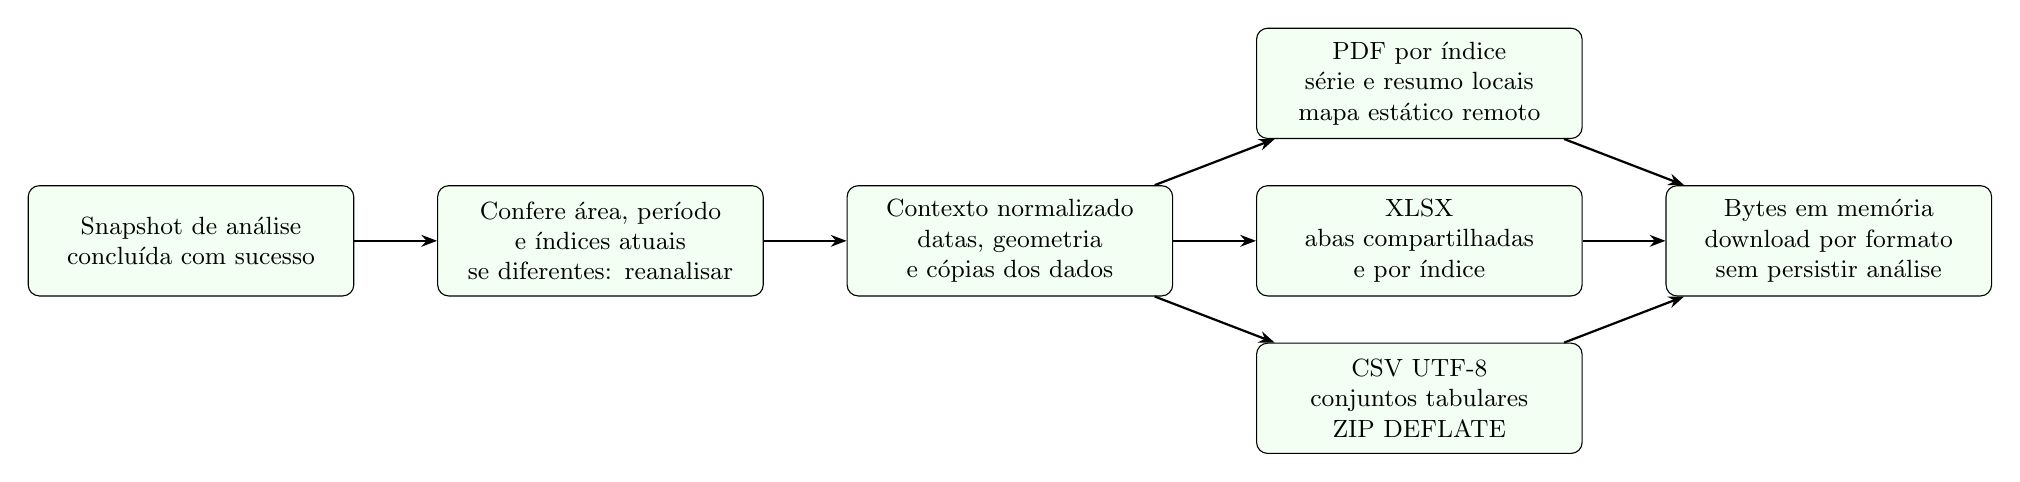
\begin{tikzpicture}[
 box/.style={draw,rounded corners,align=center,text width=39mm,
 minimum height=14mm,font=\small,fill=green!5},
 link/.style={-{Stealth[length=2mm]},thick}]
\node[box] (snapshot) at (0,0) {Snapshot de análise\\concluída com sucesso};
\node[box] (match) at (5.2,0) {Confere área, período\\e índices atuais\\se diferentes: reanalisar};
\node[box] (context) at (10.4,0) {Contexto normalizado\\datas, geometria\\e cópias dos dados};
\node[box] (pdf) at (15.6,2) {PDF por índice\\série e resumo locais\\mapa estático remoto};
\node[box] (xlsx) at (15.6,0) {XLSX\\abas compartilhadas\\e por índice};
\node[box] (zip) at (15.6,-2) {CSV UTF-8\\conjuntos tabulares\\ZIP DEFLATE};
\node[box] (download) at (20.8,0) {Bytes em memória\\download por formato\\sem persistir análise};
\draw[link] (snapshot)--(match);
\draw[link] (match)--(context);
\draw[link] (context)--(pdf);
\draw[link] (context)--(xlsx);
\draw[link] (context)--(zip);
\draw[link] (pdf)--(download);
\draw[link] (xlsx)--(download);
\draw[link] (zip)--(download);
\end{tikzpicture}
}
\caption{Geração sob demanda de arquivos a partir do snapshot de análise. Fonte: elaborado pelo autor a partir dos módulos de exportação.}
\label{fig:fluxo-exportacao}
\end{figure*}

Os formatos estruturados favorecem reutilização em ferramentas externas, inspeção dos resultados e transparência. Sua contribuição à reprodutibilidade é parcial: o contexto não inclui obrigatoriamente todos os IDs de imagens, versões de catálogo, parâmetros de reprojeção, máscaras efetivas e respostas remotas. A exportação de tabelas não constitui um pacote autossuficiente para repetir integralmente a análise.

\section{Apresentação da plataforma desenvolvida}\label{chap:plataforma-final}

\subsection{Organização e entrada espacial}

A exploração de uma região começa pela definição da área e do período. A interface reúne busca, datas, índices e acionamento da análise em torno do mapa, que recebe a demarcação antes do processamento e apresenta a composição temática depois dele. Esse fluxo permite consultar os produtos sem que o usuário tenha de manipular diretamente os arquivos raster.

\capturatcc{cap01_interface}{CAP-01}{Interface inicial, com controles analíticos e mapa de seleção}{}
\capturatcc{cap02_busca}{CAP-02}{Busca geográfica por Passo Fundo e enquadramento do mapa-base}{}

A busca resolve um nome de lugar e aproxima a navegação da região desejada, sem identificar automaticamente limites cadastrais. O mapa-base é distinto da imagem Sentinel-2 utilizada nos cálculos; sua atribuição acompanha a visualização.

A demarcação fornece a geometria das consultas. Área em hectares, perímetro e centroide permitem conferir o recorte espacial; não são estimativa de área cultivada. O salvamento associa nome e polígono, e a restauração permite repetir análises com outra configuração temporal sem redesenhar a região.

\capturatcc{cap03_poligono}{CAP-03}{Polígono demonstrativo e contexto de seleção espacial}{}
\capturatcc{cap04_salvar}{CAP-04}{Associação de nome à geometria em diálogo de salvamento}{}
\capturatcc{cap05_restaurar}{CAP-05}{Localização restaurada para reutilização da geometria}{}

O armazenamento web está vinculado à sessão. A transferência GeoJSON oferece continuidade por arquivo: exporta localizações e permite importar conjuntos validados, preservando as restrições de tamanho e quantidade. A demonstração exportou a localização e a importou em uma nova sessão. Essa estratégia não representa sincronização autenticada entre dispositivos.

\capturatcc{cap06_geojson}{CAP-06}{Transferência de localizações em GeoJSON}{}

\subsection{Configuração e produtos analíticos}

As datas inicial e final são inclusivas em UTC. A opção ``Todos'' compartilha coleção e clima entre os três índices; a alternância posterior de visualização não solicita novo processamento. A mudança de geometria, período ou conjunto analítico invalida produtos incompatíveis, mantendo a coerência da apresentação.

\capturatcc{cap07_parametros}{CAP-07}{Geometria e parâmetros da demonstração multiíndice}{}
\capturatcc{cap08_painel}{CAP-08}{Painel de resultados da análise multiíndice}{}

O painel reúne média espacial da composição, área, tendência e visão geral por indicador. A contagem corresponde às imagens filtradas, não a dias sem nuvens ou observações válidas em todos os pixels. NDWI e NDMI do sistema são variantes NIR--SWIR próximas, diferenciadas pela banda NIR empregada.

Os mapas representam a mediana temporal por posição. O gradiente permite explorar contrastes internos, e a legenda recebe os mesmos extremos da camada. A cor resume um indicador contínuo, sem atribuir automaticamente classes agronômicas.

\capturatcc{cap09_ndvi}{CAP-09}{Composição mediana NDVI da área demonstrativa}{}
\capturatcc{cap10_ndwi}{CAP-10}{Composição NIR--SWIR B8/B11, denominada NDWI no sistema}{}
\capturatcc{cap11_ndmi}{CAP-11}{Composição NIR--SWIR B8A/B11, denominada NDMI no sistema}{}

\subsection{Exploração espacial, temporal e meteorológica}

A consulta por posição permite examinar diferenças dentro da área ao apresentar o valor de uma célula da composição já transferida. Movimento e toque utilizam a mesma consulta local no navegador, com mensagens para posições fora da geometria, sem dado ou além da matriz. As quatro casas decimais são uma escolha de apresentação, não uma medida de precisão agronômica.

\capturatcc{cap12_cursor}{CAP-12}{Leitura local de célula na composição por posição}{}

Enquanto o mapa resume o período, a série temporal apresenta a média espacial de cada aquisição. O gráfico une os pontos por segmentos de reta, mas a aplicação não calcula valores diários intermediários nem elimina datas repetidas. A lista de anomalias informa as quedas sinalizadas em relação à janela anterior, ou a ausência de sinalizações. Esses recursos permitem examinar mudanças na série, sem classificar doenças ou identificar suas causas.

\capturatcc{cap13_series}{CAP-13}{Série temporal de médias espaciais e estado de sinalização}{}
\capturatcc{cap14_anomalias}{CAP-14}{Apresentação das sinalizações de desvio temporal}{}

O gráfico climático combina precipitação em barras e temperatura média em linha, com eixos próprios. Cartões resumem o período disponível. A radiação utiliza a unidade normalizada e permanece indisponível quando não há valor válido. O modo multiíndice recupera o contexto compartilhado, sem repetir a consulta para cada indicador.

\capturatcc{cap15_clima}{CAP-15}{Contexto NASA POWER, incluindo estados de disponibilidade}{}

\subsection{Relatórios e interoperabilidade}

A interface distingue preparação e download dos arquivos. O PDF sintetiza resultados visuais, o XLSX organiza abas e o ZIP distribui tabelas CSV. A geração utiliza o snapshot concluído; não recalcula os índices para cada formato. O mapa estático do PDF usa escala fixa $[-1,1]$, comunicada em sua legenda, podendo diferir do contraste ajustado do mapa interativo.

\capturatcc{cap16_exportacao}{CAP-16}{Preparação e disponibilização dos arquivos da análise}{}
\capturatcc{cap17_pdf}{CAP-17}{Relatório PDF efetivamente gerado pela análise}{}
\capturatcc{cap18_xlsx}{CAP-18}{Organização tabular dos resultados exportados}{}
\capturatcc{cap19_zip}{CAP-19}{Conteúdo CSV distribuído no arquivo ZIP}{}

As saídas permitem conferir e reutilizar informações fora da interface, mas não incluem raster GeoTIFF nem toda a proveniência necessária para reconstruir exatamente o processamento remoto. Os arquivos XLSX e ZIP da demonstração foram verificados programaticamente; suas capturas em visualizadores próprios permanecem pendentes e, por isso, não são apresentadas como evidência visual concluída.

\subsection{Adaptabilidade e acesso público}

O CSS possui regras para larguras até 1.100, 768 e 480 pixels, reorganizando os controles. Mapas e gráficos integram o layout web, não um aplicativo móvel nativo. O tratamento de toque amplia a exploração sem cursor, mas desenho, importação e downloads também dependem do navegador e do sistema operacional. Uma execução em viewport móvel não equivale a teste em telefone físico.

\begin{figure}[htbp]
\centering
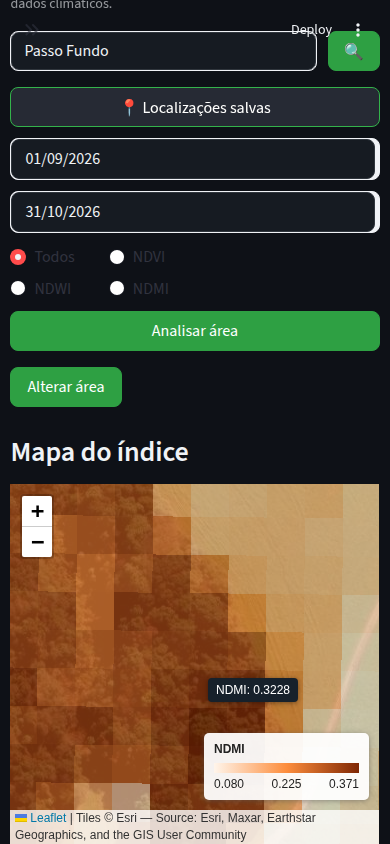
\includegraphics[width=0.74\columnwidth,height=0.43\textheight,keepaspectratio]{fig/capturas/mobile_resultados.png}
\caption{Consulta por toque e legenda NDMI em área de visualização de 390 $\times$ 844 pixels. Emulação em Chrome, não telefone físico. Fonte: captura real da aplicação local.}
\label{fig:mobile}
\end{figure}

A aplicação pode ser acessada sem instalação local pelo visitante no \href{https://eduardo198272-monitoramento-agricola-satel-streamlit-app-q0mow9.streamlit.app/}{endereço público Streamlit}. O QR Code da \cref{fig:qr-acesso} aponta para o URL completo e foi conferido por decodificação. A verificação de acesso não implica disponibilidade contínua nem publicação das correções locais.

\begin{figure}[htbp]
\centering

\includegraphics[width=0.48\columnwidth]{fig/qr_plataforma.png}
\caption{QR Code de acesso ao endereço público. Fonte: elaborado pelo autor.}
\label{fig:qr-acesso}
\end{figure}

\section{Resultados}\label{chap:resultados-final}

\subsection{Artefato desenvolvido}

A plataforma integra seleção e reutilização de geometrias, processamento Sentinel-2, exploração espacial, séries, contexto meteorológico e resultados portáveis. O processamento remoto evita manter o acervo orbital no servidor da aplicação; o pré-carregamento raster permite consulta numérica no navegador. Armazenamento local e isolamento por sessão atendem a contextos distintos, complementados por transferência GeoJSON.

\subsection{Avaliação computacional}

A versão avaliada corresponde à base \texttt{b7c325c} acrescida das alterações locais documentadas. Em Linux x86\_64, Python 3.14.4, pytest 9.0.3 e tracer C, o comando \texttt{python -m pytest -q -p no:cacheprovider}, com \texttt{COVERAGE\_CORE=ctrace}, aprovou \textbf{710 testes em 11,73 s}, sem falhas ou testes ignorados. A cobertura em \texttt{src/app} foi de \textbf{100\% das linhas e ramificações}, com 2.735 instruções e 856 ramificações, sem caminhos parcialmente cobertos. A linha de base de 686 testes permaneceu preservada; novos casos verificaram os contratos corrigidos.

Os testes abrangem regras locais, integração entre módulos, persistência temporária, widgets Streamlit e serialização. Serviços remotos são substituídos em parte da suíte. A medição não inclui o ponto de entrada da raiz nem HTML/JavaScript. Separadamente, três testes Node verificaram legenda negativa, lookup de células e NoData, e descompressão zlib/Base64 em \texttt{Float32Array}; os três foram aprovados. Esses testes não constituem uma matriz de compatibilidade de navegadores.

Cobertura integral indica execução dos caminhos medidos, não ausência de defeitos. A avaliação dos contratos encontrou suposições semânticas que a suíte anterior não distinguia, motivando regressões específicas sem reduzir a meta.

\subsection{Verificação das integrações}\label{sec:resultado-unidades}

Uma resposta pública NASA POWER, preservada para longitude $-52$ e latitude $-28$ entre 01/01/2025 e 02/01/2025, declara radiação em MJ/m²/dia e valores 21,64 e 20,99. A média é 21,315. A conversão anterior multiplicava essa média por 3,6, produzindo 76,734 sob o mesmo rótulo. A normalização pelos metadados passou a preservar MJ e converter somente kWh declarados. Testes verificaram a média corrigida, as duas linhas XLSX/CSV e a representação resumida do PDF.

A avaliação também harmonizou limites temporais, resumo meteorológico compartilhado e metadados dos pipelines. Um teste multiíndice confirmou uma única obtenção do contexto climático. Outro distinguiu aquisições do mesmo dia na marcação de anomalias. Alterações analíticas passaram a invalidar todos os produtos derivados, enquanto a troca visual entre índices calculados preserva a análise.

No mapa, o mesmo intervalo usado nos tiles é enviado à legenda. A escala fixa do PDF permanece uma escolha separada, comunicada no próprio produto. A correção do contrato não implica igualdade pixel a pixel entre reduções remotas, grade reamostrada e mapa estático.

\subsection{Demonstração funcional}

Uma sessão real em Chrome confirmou o fluxo entre busca por Passo Fundo, demarcação, salvamento, restauração, análise e download. O recorte demonstrativo de aproximadamente 4,36 ha foi consultado entre 01/09/2026 e 31/10/2026, sem atribuição de cultura ou propriedade. Duas imagens passaram pelos filtros, em 08/09 e 20/10. As médias espaciais das composições foram 0,7070 (NDVI), 0,2140 (NDWI) e 0,2380 (NDMI). Esses valores caracterizam o exemplo computacional, não uma amostra representativa de áreas agrícolas.

As séries contiveram dois pontos por índice, insuficientes para a janela de três observações anteriores do detector; a ausência de anomalias nessa demonstração não informa eficácia de detecção. O clima apresentou 61 registros, precipitação acumulada de 635,56 mm e temperatura média de 16,24 °C. A radiação permaneceu indisponível e foi mantida ausente nos arquivos, sem preenchimento por suposição.

O PDF baixado contém três páginas com mapas estáticos, o XLSX possui sete abas e o ZIP sete arquivos CSV com integridade estrutural conferida. O identificador de aquisição está presente nas séries tabulares. A consulta NDMI na posição $(-52{,}331,-28{,}228)$ exibiu 0,3228, tanto por movimento quanto por toque em viewport de 390 pixels. O resultado pertence à célula reamostrada da composição e não substitui a média espacial de 0,2380.

O endereço público respondeu HTTP 200 e apresentou a interface Streamlit em navegador. Essa verificação não estabelece equivalência entre versão publicada e alterações locais nem disponibilidade contínua. As capturas analíticas correspondem à execução local corrigida; manifestos e arquivos preservam o vínculo com os parâmetros.

\subsection{Avaliação com usuários}

O instrumento está disponível para participação voluntária, conforme a \cref{sec:pesquisa-usuarios}. Não foi disponibilizado um conjunto de respostas reais para esta análise; por isso, não são apresentados tamanho amostral, avaliações, gráficos ou depoimentos. O procedimento reproduzível foi preparado e testado com entradas sintéticas isoladas, que não integram os resultados da pesquisa.

\section{Discussão}\label{chap:discussao-final}

\subsection{Atendimento aos objetivos e evolução do escopo}

Os objetivos de integração, seleção de áreas, índices, mapas, séries e exportação foram materializados em módulos verificáveis. A \cref{tab:objetivos-final} distingue implementação e extensão da avaliação, sem equiparar testes de software a estudos agronômicos.

\begin{table*}[htbp]
\centering\small
\caption{Síntese do atendimento aos objetivos da redação final.}
\label{tab:objetivos-final}
\begin{tabular}{p{0.10\textwidth}p{0.20\textwidth}p{0.61\textwidth}}
\hline
\textbf{Objetivo} & \textbf{Situação} & \textbf{Fundamento e ressalva} \\ \hline
OE1 & Implementado & Estrutura modular e métodos documentados; bibliografia com pendências explícitas. \\
OE2 & Implementado & Busca, desenho, gravação e recuperação; sessão web não é persistência permanente. \\
OE3 & Implementado & Filtros e fórmulas exercitados, demonstração remota executada; adequação histórica da máscara requer avaliação específica. \\
OE4 & Implementado & Composição, média e consulta local; contrato de escala corrigido e testado. \\
OE5 & Implementado & Série, tendência e regra unilateral exercitadas com dados controlados; sem acurácia agronômica atribuída. \\
OE6 & Implementado & Clima compartilhado, unidade normalizada e resumo propagado; ausência tratada explicitamente. \\
OE7 & Implementado & PDF, XLSX, CSV ZIP e GeoJSON exercitados com entradas controladas; não equivalem a pacote completo de reprodução. \\
OE8 & Parcialmente concluído & Suíte e fluxo real com downloads executados; pesquisa com usuários sem resultados e estudos por cultura não realizados. \\ \hline
\end{tabular}
\end{table*}

Na proposta, NDVI e NDWI eram o foco e NDMI aparecia como evolução futura. A implementação incorporou NDMI, exploração numérica no navegador, modos de armazenamento e exportações estruturadas. A ausência original de banco foi substituída por SQLite local e, posteriormente, por alternativa de sessão para o ponto de entrada web. Essas adições são resultados de engenharia e não substituem o objetivo original de validar o protótipo em áreas de soja, milho e pastagem.

Os estudos de soja, milho e pastagem, experimentos controlados e coleta em campo previstos não foram realizados. A avaliação concentrou-se no artefato computacional. Essa delimitação mantém a contribuição de engenharia, mas não substitui o objetivo experimental original e requer apreciação do orientador.

Outros requisitos das especificações também exigem distinção. O fluxo atual mostra área em hectares, sem seletor de acres, e não implementa bloqueio/liberação explícitos de navegação como descrito em especificações anteriores. A exclusão de localizações está no serviço, mas não na interface. Descrever esses itens como integralmente disponíveis apenas porque constam no planejamento produziria uma representação inadequada do sistema.

\subsection{Contribuições de Engenharia de Software}

A plataforma articula representações heterogêneas: texto de busca, coordenadas, polígonos, operações remotas de imagem, matrizes comprimidas, séries e arquivos. O encapsulamento em serviço e repositórios permite manter as regras de nome e transferência independentemente do armazenamento local ou de sessão. O snapshot de exportação reduz a possibilidade de gerar arquivos associados a parâmetros diferentes dos que produziram os dados.

O componente de consulta local é uma decisão de interação relevante: transfere uma grade após a análise para evitar requisições por movimento do cursor. Em contrapartida, impõe custo de memória e transferência, depende de suporte do navegador e limita o tamanho da região. Trata-se de um compromisso explícito de engenharia, não de comprovação de baixa latência em qualquer área.

As exportações disponibilizam informações fora da interface e permitem conferir dados com outras ferramentas. O PDF sintetiza, enquanto tabelas e GeoJSON preservam estruturas reutilizáveis. Contudo, não há exportação de toda a proveniência necessária à reconstrução exata do processamento. Interoperabilidade e transparência são ampliadas, mas reprodutibilidade integral ainda requer versões, IDs, parâmetros e dados auxiliares adicionais.

\subsection{Consistência das integrações e limites dos testes}

A divergência corrigida na radiação evidencia a diferença entre cobertura e correção semântica: a execução dos caminhos não verifica, por si só, a unidade de origem. A interpretação explícita dos metadados e sua reutilização em resumo e exportações reduziram a duplicação dessa regra.

A legenda passou a compartilhar o intervalo dos tiles. O mapa interativo favorece contraste interno ao recorte, enquanto o PDF mantém escala fixa, útil para referência comum entre relatórios. Aparências distintas podem ser corretas quando cada escala é comunicada.

A harmonização dos pipelines e a associação por aquisição preservam a interpretação dos registros entre modos e formatos. O identificador melhora a proveniência tabular, embora ainda não constitua inventário completo de processamento. A invalidação de estado complementa esse cuidado ao impedir apresentação de resultados sob parâmetros analíticos diferentes.

\subsection{Limitações espaciais, temporais e estatísticas}

A máscara QA60 não resolve todos os problemas de nuvens e sombras e possui restrições históricas de disponibilidade. O filtro de nuvens é do produto, não da área. A grade a 10 m não confere resolução nativa de 10 m às bandas B8A e B11. A média espacial do pipeline não fixa explicitamente o CRS, enquanto a consulta interativa utiliza UTM; correspondência numérica estrita requer verificação adicional.

A composição mediana pode reduzir a influência de observações extremas, mas também oculta quando uma mudança ocorreu e quantas observações sustentam cada posição. A série pode apresentar lacunas, datas repetidas e variação do suporte espacial válido. O resumo de imagens não informa essa cobertura por pixel.

A heurística de anomalias considera apenas três observações e desvios negativos. Não sinaliza quedas após janela de desvio zero, não modela sazonalidade ou fenologia e não separa ruído de mudanças reais. A tendência usa ordem de observações, não tempo decorrido. Sem referências agronômicas e avaliação apropriada, esses produtos servem à exploração de comportamentos atípicos e não ao diagnóstico automático.

\subsection{Operação, serviços e avaliação não realizada}

O uso de bibliotecas abertas deve ser distinguido do acesso a serviços externos. Earth Engine e Esri não são componentes locais de código aberto da aplicação. Dados Sentinel possuem condições próprias de uso, o serviço de geocodificação público possui política de utilização e o Earth Engine requer projeto e elegibilidade, com cotas e condições específicas \citep{GOOGLE_EE_NONCOMMERCIAL,NOMINATIM_POLICY}. Não se demonstrou operação comercial gratuita ou custo total inferior ao de outras soluções.

O serviço público Nominatim limita o tráfego agregado da aplicação a uma requisição por segundo e proíbe autocomplete. O código utiliza busca explícita e identifica a aplicação, mas não implementa limitador global ou cache de buscas. A atribuição e as condições de acesso devem ser revistas antes de ampliar o número de visitantes; disponibilidade pública não implica capacidade ilimitada.

Na web, visitantes compartilham a conta de serviço e o consumo de cotas, embora os registros estejam separados por sessão. GeoJSON e arquivos de resultados podem conter coordenadas sensíveis, e a privacidade dos arquivos transferidos fica sob responsabilidade de quem os armazena e compartilha. O isolamento de sessão não constitui sistema de autorização de propriedades.

Não foram conduzidos testes de carga, ensaios representativos de latência, comparação quantitativa com plataformas ou avaliação de campo. A pesquisa de experiência de uso permanece sem resultados analisados; sua amostragem por adesão limitará generalizações. A resolução das bandas e dos dados meteorológicos, a dependência de serviços e cotas, a memória da grade no navegador e a natureza heurística das anomalias delimitam o uso. A máscara QA60 foi preservada: uma substituição por SCL ou probabilidade de nuvens exige verificação de classes, sombras, disponibilidade histórica e efeitos sobre os resultados, não apenas troca de API.

A inspeção visual identificou contraste insuficiente em alguns textos quando os estilos escuros se combinam ao tema de widgets do ambiente. A emulação móvel confirmou reorganização e lookup por toque, mas não substitui ensaios de acessibilidade ou uma matriz de dispositivos e navegadores.

\section{Conclusão}\label{chap:conclusao-final}

O trabalho materializa uma plataforma computacional que reúne seleção geográfica, consulta a imagens, índices espectrais, séries temporais, contexto climático e exportação de resultados. A evolução para execução web preserva o SQLite local e adiciona isolamento de sessões e transferência GeoJSON, sem introduzir banco externo ou login de visitantes.

Os 677 testes aprovados, a cobertura integral dos módulos medidos com tracer C e a verificação mínima de acesso real ao Earth Engine constituem evidências de software, não validação agronômica. Em resposta à pergunta de pesquisa, a implementação demonstra uma forma de integrar os componentes e verificar seus contratos; a avaliação da plataforma como ferramenta de monitoramento agrícola ainda requer execução documentada de ponta a ponta e conferência independente dos cálculos.

Permanecem como próximos passos a validação da publicação no Streamlit Cloud, os cenários com culturas e geometrias confirmadas e as verificações de máscaras, resoluções e unidades climáticas. Até a obtenção dessas evidências, esta conclusão é parcial e não reivindica eficácia em campo, superioridade sobre outras ferramentas ou estudo de usabilidade concluído.

% PENDENTE: sintetizar o atendimento dos objetivos após a avaliação documentada.
% PENDENTE: apresentar contribuições efetivamente demonstradas, limitações e trabalhos futuros coerentes com os resultados.

\bibliography{referencias}
\end{document}
